\documentclass[11pt,a4paper]{report}

\usepackage{array}
\usepackage{graphicx}
\graphicspath{ {./images/} }

% Aberstwyth MMP Project Report Template for LaTeX
%
% Authors: Neil Taylor (nst@aber.ac.uk) and Dr. Hannah Dee (hmd1@aber.ac.uk) 
%
% This has been adapted from the Leeds Thesis template and the 
% Group Project template for Computer Science in Aberystywth University.
% 
% All comments and suggestions welcome.
%
% Template designed to be used with pdflatex: it may need alteration to
% run with a different LaTeX engine.
%
% Note - this is offered as a starting point for your work. You are not 
% required to use this template and can choose to create your own document 
% without it.

% This template is suitable for students with an engineering-style project, 
% which will be most students in the department. If your project is a research-oriented 
% project, look at the alternative template.

% To build document on the unix command line, run four commands:
 
% pdflatex mmp-report
% bibtex mmp-report
% pdflatex mmp-report
% pdflatex mmp-report

% you will end up with mmp-report.pdf. Before submitting, add your user ID as a prefix, 
% e.g. abc01-mmp-report.pdf 
\usepackage{StylesAndReferences/mmp-report}

% the following packages are used for citations - You only need to include one. 
%
% Use the cite package if you are using the numeric style (e.g. IEEEannot). 
% Use the natbib package if you are using the author-date style (e.g. authordate2annot). 
% Only use one of these and comment out or remove the other one. 
\usepackage{cite}
%\usepackage{natbib}

%%%% Title and Section Colours %%%%
% Modify these values to change the colours used for title, sections and subsections.
% Each value is a range of 0-255 in RGB colourspace.
% Idea courtesy of discussion at 
% https://www.overleaf.com/learn/latex/Using_colours_in_LaTeX
% and
% https://tex.stackexchange.com/questions/75667/change-colour-on-chapter-section-headings-lyx
% 
% If you prefer to have black headers, then comment out the following lines
\definecolor{mmpTitle}{RGB}{10, 85, 145}
\definecolor{mmpSection}{RGB}{10,85,155}
\definecolor{mmpSubsection}{RGB}{79,129,189}

\chapterfont{\color{mmpTitle}}  % sets colour of chapters
\sectionfont{\color{mmpSection}}  % sets colour of sections 
\subsectionfont{\color{mmpSubsection}} % sets colour subsections
\subsubsectionfont{\color{mmpSubsection}} % sets colour subsections

%%%% end of Title and Section Colours %%%%


%%%% Report Type %%%%
%% comment/uncomment depending on the type of report you want to generate
\reporttype{Engineering}
%\reporttype{Research}
%%%% end of Report Type %%%%


\begin{document}

%TC:ignore

% all of the include directives below refer to tex files
% so %TC:ignore 

\title{Customisable non-graphical interface to start/stop activities on mobile robots}

% Your name
\author{Sam Matthews}

% Your email 
\authoremail{sam82@aber.ac.uk}

\degreeschemecode{GH76} %e.g. G400 
\degreeschemetitle{Artificial Intelligence And Robotics} % e.g. Computer Science
\degreetype{BSc}

\modulecode{CS39440} % i.e. CS39440, CC39440, CS39620
\moduletitle{Major Project} % i.e. Major Project or Minor Project

\date{3rd May 2019} % i.e. the date of the current version of your report

\status{Release} % Use draft until you create the release version. Then, change this to Release.
\version{1.0}

% The title and name of your supervisor.
\supervisor{Dr. Frédéric Labrosse} 

%The email for your supervisor. 
\supervisoremail{ffl@aber.ac.uk}

\maketitle

%TC:endignore
 includes cover.tex - to change the content,
% edit the tex file

\pagenumbering{roman}

% This is the front page
%TC:ignore 

\title{Customisable non-graphical interface to start/stop activities on mobile robots}

% Your name
\author{Sam Matthews}

% Your email 
\authoremail{sam82@aber.ac.uk}

\degreeschemecode{GH76} %e.g. G400 
\degreeschemetitle{Artificial Intelligence And Robotics} % e.g. Computer Science
\degreetype{BSc}

\modulecode{CS39440} % i.e. CS39440, CC39440, CS39620
\moduletitle{Major Project} % i.e. Major Project or Minor Project

\date{3rd May 2019} % i.e. the date of the current version of your report

\status{Release} % Use draft until you create the release version. Then, change this to Release.
\version{1.0}

% The title and name of your supervisor.
\supervisor{Dr. Frédéric Labrosse} 

%The email for your supervisor. 
\supervisoremail{ffl@aber.ac.uk}

\maketitle

%TC:endignore
                        

% Set up page numbering
\pagestyle{empty}

% declarations of originality 
\thispagestyle{empty}

%TC:ignore

%%%
%%% You must sign the declaration of originality. 
%%%
%%% You are submitting this electronically. Therefore, to sign, you 
%%% type your name and date to replace the .... characters. 
%%%
\section*{\centering Declaration of originality}

I confirm that:

\begin{itemize}
\item{This submission is my own work, except where 
clearly indicated.}

\item{I understand that there are severe penalties for Unacceptable Academic Practice, which can lead to loss of marks or even the withholding of a degree.}
 
\item{I have read the regulations on Unacceptable Academic Practice from the University's Academic Registry (AR) and the relevant sections of the current Student Handbook of the Department of Computer Science.}
 
\item{In submitting this work I understand and agree to abide by the University's regulations governing these issues.}
\end{itemize}

\vspace{2em}
Name Sam Matthews \\

\vspace{1em}
Date 3rd May 2019 \\

%%% 
%%% We would like to make a selection of final reports available to students that take 
%%% this module in future years. To enable us to do this, we require your consent. You 
%%% are not required that you do this, but if you do give your consent, then we will have 
%%% the option to select yours as one of a number of reports as examples for other 
%%% students. If you would like to give your consent, then please include the following 
%%% text and type your name and date to replace the .... characters. 
%%% 
%%% If you do not wish to give your consent, please remove this from your report. 
%%%
%\vspace{1em}
%\section*{\centering Consent to share this work}

%By including my name below, I hereby agree to this project's report and technical work being made available to other students and academic staff of the Aberystwyth Computer Science Department.  

%\vspace{2em}
%Name ............................................................  \\

%\vspace{1em}
%Date ............................................................ \\

%TC:endignore

               

\thispagestyle{empty}

%TC:ignore

\section*{\centering Acknowledgements}

I would like to thank my supervisor Fred Labrosse for his support throughout the entire project.

%I would also like to thank my parents for listening to me as I descend into madness.

%TC:endignore
 % Acknowledgements

\thispagestyle{empty}

%TC:ignore

\section*{\centering Abstract}

The main goal of this project was to solve various problems associated with operating the large robots in the department. These robots have screens attached to them that display a non-graphical environment running Linux and can be controlled using mounted keyboards. The most notable problem with this is that the output of only one process can be monitored in a single {\fontfamily{pcr}\selectfont TTY}, meaning that it was necessary to log in to separate {\fontfamily{pcr}\selectfont TTY} instances. Additionally, using an entirely terminal-based interface is inconvienient due to the necessity to type every command. To streamline this process, it seemed appropriate to create a "tabbed" interface that allows users to run commands from a list as well as switch between different processes using a tab bar. This can run any executables including {\fontfamily{pcr}\selectfont ROS} nodes that are defined in a configuration file beforehand. In addition to this, it was also decided to include a method for teleoperation within the application as well as a configurable way to display {\fontfamily{pcr}\selectfont ROS} topics in a menu. The main outcome of this work is a form of convienience and flexibility for anyone performing experiments using the robots and provides a form of redundancy in the event that a laptop connected to the robot is unavailable/infeasable.

%TC:endignore
                 % Abstract

\pagenumbering{roman}
\pagestyle{fancy}
\fancyhead{}
\fancyfoot[C]{\thepage}
\renewcommand{\headrulewidth}{0 pt}
\renewcommand{\chaptermark}[1]{\markboth{#1}{}}

\tableofcontents   
\newpage
\listoffigures % comment out this line if you don't have any figures / graphics
\newpage 
\listoftables % comment out this line if you don't have any tables
\newpage

% Set up page numbering
\pagenumbering{arabic}

\setchapterheaderfooter

%TC:endignore

% include the chapters
\chapter{Background \& Objectives}

\section{Background}

The main objective of this work was to provide an application for operating robots that emphasised efficient use of resources as well as usability. The personal motivation for this project was to create something that can have a real benefit towards future research and will actually be used by others in their own work to make their lives easier/better. This is in addition to personal interest and experience in using low level, non-graphical applications that emphasise speed, extensibility and usability. This project provided an opportunity to understand how these sorts of systems work as well as the potential to make more of these types of systems.

\subsection{Similar Systems}
\label{similar}

There are plentiful and various open source systems to assess in order to gain an understanding of non-graphical applications. One example that was assessed was {\fontfamily{pcr}\selectfont tmux}\cite{tmux}, a terminal multiplexer written in {\fontfamily{pcr}\selectfont C} using {\fontfamily{pcr}\selectfont ncurses}. This application runs in the terminal and can divide a terminal window into tiles running separate shell sessions. It can also display different "windows" which are similar to virtual workspaces and displays tabs at the bottom of the screen to represent these workspaces. This demonstrated the possibilities regarding the monitoring of program output and preserving it in tabs. The main problem with {\fontfamily{pcr}\selectfont tmux} as an alternative is that there is no menu to select applications to run from built in as each window is a shell prompt.

Another example that was looked at was {\fontfamily{pcr}\selectfont ranger}\cite{ranger}, a terminal file manager written in {\fontfamily{pcr}\selectfont Python} using the {\fontfamily{pcr}\selectfont curses} module. {\fontfamily{pcr}\selectfont Ranger} shows a usage of menus that can be navigated using key bindings as well as mouse input. Similarly to {\fontfamily{pcr}\selectfont tmux}, {\fontfamily{pcr}\selectfont ranger} divides the terminal into sections and has "tabbed" functionality. However, unlike {\fontfamily{pcr}\selectfont tmux}, the sections show menus that display the current and parent directory as well as a preview of the currently selected file/directory. Also, the tabs are essentially different {\fontfamily{pcr}\selectfont ranger} sessions that help to multi-task within the same window. The general layout of {\fontfamily{pcr}\selectfont ranger} is very intuitive for this kind of application and also demonstrates further possibilities in terms of capturing process output and manipulating text.

Finally, a system that is already being used for controlling these robots is a {\fontfamily{pcr}\selectfont qt} application made by Fred Labrosse. This application has dedicated tabs for stopping, teleoperation and status monitoring. This application was the basis of what this project is trying to recreate in the terminal aside from some extra features. As a result, the layout and functionality of the relevant sections of my application are very similar to his.

\subsection{Reading and Preparation}
\label{reading_and_prep}

The initial preparation for this project involved considering the various ways to make a non-graphical application. Creating a custom UI library would have been infeasible so utilising existing tools was necessary. A very common tool for this is {\fontfamily{pcr}\selectfont ncurses}\cite{ncurses}, however, alternative tools were considered such as {\fontfamily{pcr}\selectfont termbox}\cite{termbox} and even {\fontfamily{pcr}\selectfont BASH}\cite{bash-tui}.

The Curses Development Environment (CDK)\cite{cdk} was also tested in order to make the design less complex. This library adds {\fontfamily{pcr}\selectfont ncurses} widgets such as menus and buttons and can help to construct a TUI much quicker. Unfortunately, this did not work during initial testing and so was disregarded in favour of writing similar code from scratch. Additionally, there is no tab bar widget included meaning that some of the UI would have to be hand coded regardless.

The primary reading for this area mostly consists of reading manual pages for standard Unix utilities. There are some exceptions such as this comprehensive guide on {\fontfamily{pcr}\selectfont ncurses}\cite{ncurses-howto}. Some prototypes were made in order to get a better understanding of the admittedly sparse documentation. Additionally, this work illustrated how {\fontfamily{pcr}\selectfont ncurses} works in terms of displaying text which informed later design decisions.

As preparation for the report, a journal was kept and updated daily indicating progess and difficulties. This also acted as a way to organise new features to add based upon weekly meetings. This journal was not written as a blog and is not publicly available.

\section{Analysis}
%Taking into account the problem and what you learned from the background work, what was your analysis of the problem? How did your analysis help to decompose the problem into the main tasks that you would undertake? Were there alternative approaches? Why did you choose one approach compared to the alternatives? 

%There should be a clear statement of the objectives of the work, which you will evaluate at the end of the work. 

%In most cases, the agreed objectives or requirements will be the result of a compromise between what would ideally have been produced and what was determined to be possible in the time available. A discussion of the process of arriving at the final list is usually appropriate.

The background work resulted in the selection of {\fontfamily{pcr}\selectfont ncurses} as the method of creating a non-graphical interface. This was decided as {\fontfamily{pcr}\selectfont ncurses} is a standard utility used everywhere and has more useful features than the more minimalist alternatives such as built in panes for splitting the terminal window. It is also the same tool used by the similar systems that were assessed. This will allow the application to be run in most terminal emulators as well as the {\fontfamily{pcr}\selectfont TTY}.

Due to the low-level nature of {\fontfamily{pcr}\selectfont ncurses}, there was an understanding that not many UI features would be implemented. This is because more is required in order to achieve similar results in a more graphical API. This analysis showed that the final system had to be relatively simple so that other requirements could be feasibly met within the scope of the project.

\subsection{User Stories}
\label{user_stories}

The requirements were identified as user stories after the background work was done and a better understanding of the project had been achieved. The stories that were identified are as follows:

\begin{itemize}
  \item The main menu is generated from a configuration file that the user can specify.
  \item The user can run processes by selecting them from the menu. The process will appear in a tab and the output is displayed in the main window.
  \item The user can switch tabs to view different processes being outputted.
  \item Users can close the currently views process which kills it and removes it from the tab bar.
  \item The user can scroll through menu items or output using a scrollbar. This behaviour is based on the size of the window and the limit of the buffer.
  \item The robot can be controlled by the user using the keyboard or touch screen
  \item There will be a part of the interface that will display robot status information
\end{itemize}

Each requirement was also associated with relevant classes as depicted in the class diagram in Appendix \ref{appendix:d}.

\subsection{Project Components}

The problem was broken up into three main systems, each of which represent a distinct stage in development as well as its own set of requirements. The ordering of these sections was based mainly on personal preference towards developing a user interface before the back-end. It was also foreseen that each of theses sections would take up a similarly significant partition of the code.

\subsubsection{User Interface}

The UI was seen as a substantial component of the system as it was made up of various interconnected sub-components. For most, projects, the user interface could be considered the simplest part, however, creating a comprehensive user interface is more involved with the tools that were used. The {\fontfamily{pcr}\selectfont ncurses} library definitely makes this process simpler, however, it is still low level and more tightly integrated into the back-end. The user interface was broken up further into windows that each serve a related yet distinct purpose. The main windows consist of the main output area, the process menu and the tab bar.

\subsubsection{Process Management and Multitasking}

This section concerns the ability to run pre-defined processes from a menu and view the output of each of them. To achieve this, the application needs to keep track of all open processes as well as be able to redirect and capture output. Additionally, it should be ensured that all processes are updated at equal intervals and that there is no performance impact on the user experience. There should also be functionality for closing a process tab that would also effectively kill the process.

\subsubsection{Teleoperation and Monitoring}

Teleoperation refers to the ability to control a robot using its own keyboard. This is arguably not teleoperation as it is not remote controlled, however, it can be used as such if the application itself is run on a separate machine and publishes messages to the topic the robot is listening to. Therefore, this feature will be known and referred to as teleoperation. This will involve creating a dedicated window layout with buttons that can send different velocity messages as well as being able to control the robot using the keyboard.

The monitoring feature will have another dedicated window layout that displays status information of the robot. The topics to display will be inspired by the existing {\fontfamily{pcr}\selectfont qt} application that was assessed in Section \ref{similar}.

\subsection{Security and Safety Issues}
\label{safety}

Due to the nature of this project, there are little to no security issues as there are already security measures put into place on the robot platforms being used. Also, the application does not deal with private information nor does it interface with networking protocols at all.

However, there are certainly issues of safety to consider as this application will be directly and indirectly controlling large, heavy machinery. While this is not strictly related to security, measures still need to be taken during the project as well as considered during the design of the software. To combat these potential issues, all hardware testing is done under supervision and is accompanied by the existing teleoperation application. This is running on a laptop and can stop the robot immediately at any time in case anything goes wrong. Additionally, it is important to close programs opened in the application carefully to ensure that messages are not still being sent upon shutdown.

\section{Process}

The development process throughout the project can be described as a modified version of Scrum that is more appropriate for one individual rather than a team. This adaptation removes the idea of roles and instead allows for all work, planning and assessment to fall to a single developer as well as the client where necessary. What remains is an iterative development approach with an emphasis on rapid prototyping and integration as well as quick response to a change in the client's requirements. The justification for this approach is due to inexperience with the chosen technologies as well as the fact that the requirements were constantly subject to change.
    
Each sprint lasted for one week, at the end of which was a meeting with the project supervisor/client. This meeting would comprise of reporting progress, discussing issues and new features as well as planning the objectives for the following sprint. The start of a sprint would include either an analysis of a new feature to be completed or prioritising the most urgent/important items in the backlog. The amount of features to be completed in each sprint depends on individual understanding of personal velocity. If all designated features were finished before the end of the sprint, the next item on the backlog would be addressed.

%\addcontentsline{toc}{chapter}{Development Process}
\chapter{Overall Final Design}
\label{chapter:design}

%You should concentrate on the more important aspects of the design. It is essential that an overview is presented before going into detail. As well as describing the design adopted it must also explain what other designs were considered and why they were rejected.

%The design should describe what you expected to do, and might also explain areas that you had to revise after some investigation.

%Typically, for an object-oriented design, the discussion will focus on the choice of objects and classes and the allocation of methods to classes. The use made of reusable components should be described and their source referenced. Particularly important decisions concerning data structures usually affect the architecture of a system and so should be described here.

%How much material you include on detailed design and implementation will depend very much on the nature of the project. It should not be padded out. Think about the significant aspects of your system. For example, describe the design of the user interface if it is a critical aspect of your system, or provide detail about methods and data structures that are not trivial. Do not spend time on long lists of trivial items and repetitive descriptions. If in doubt about what is appropriate, speak to your supervisor.

%You should also identify any support tools that you used. You should discuss your choice of implementation tools - programming language, compilers, database management system, program development environment, etc.

The evolution of the design of the application is inherent to the agile methodology adopted. The design outlined in this section will illustrate the final design as well as talk about how each design element has evolved when appropriate. Some of the design has been consistent from the beginning of the project such as the general user interface design. However, other parts needed to evolve due to a change in the understanding of the requirements and the technical limitations of the technologies used. There is also discussion of some decisions made that are not relevant to the content in Chapter \ref{chapter:implementation}.

Much of the initial design consisted of user stories arranged on a story board alongside basic class descriptions. These items were arranged on the story board in such a way that the classes would cluster around relevant stories and create spatial CRC "cards".

\section{Overall Architecture}

The final design of this project uses an object oriented approach to development making use of inheritance and encapsulation. The class diagram illustrating this design is included in Appendix \ref{appendix:d}.

As is common for object-oriented programs, the main method is usually small and merely exists to construct an object that will itself run the application. Regardless of this convention, it was decided that this is wasteful and that the main function should be used appropriately. The usefulness of objects within the design is arguably restricted to the utilisation of inheritance for the front end classes. This is likely due to a personal bias towards procedural programming paradigms which is why {\fontfamily{pcr}\selectfont C} was initially used as noted in Section \ref{implementation_tools}. However, the re-implementation in {\fontfamily{pcr}\selectfont C++} affected the initial design as it was decided that making effective use of the language's features (including objects) was important, regardless of personal preference.

Each section of the screen is represented by a Window object that defines its co-ordinates as well as dictates the behaviour of printing. The Menu inherits from the Window to take advantage of the printing functionality as well as implement menu selection. The TabBar then inherits from the menu as it is effectively the same aside from the orientation and the ability to iteratively refresh processes. It seemed more appropriate to make the tab bar act as the container/manager for the running processes as opposed to having a dedicated object for such activity. This provides a way to bridge the gap between the front and back ends. The teleoperation interface was planned to inherit from the window class as this seemed to make the most sense at the time. However, it was deemed to be unnecessary as much of the functionality was unrelated to the other windows. As a result, the front end of the teleoperation system is a function in Window, whereas the back end encompasses its own independent class.

The Button class does not inherit from window even though much of its functionality is the same. The reason for this is that the window class automatically spawns with a list of buttons. This could be potentially changed to reduce duplicated code, although the benefits gained are not substantially worth it.

A class that was omitted was the ScrollBar class which would have been used for spawning and updating the scrollbars. It would also scroll through the printed output and maintain the current scrolling position. This was also found to be redundant due to the simplicity of scrolling and how easy it would be to integrate it directly into the main printing function.

The back end classes mainly consist of Monitor, Teleop and Process. The monitoring and teleoperation classes are mostly used to manage {\fontfamily{pcr}\selectfont ROS} messages in a way that can be interfaced with the from end. The process class is integral for process management and stores information about each process as well as provides tools to start/stop them.

In terms of the overall behaviour, the application is based around the main loop that accepts user input and acts accordingly. Within this loop, each refresh subroutine occurs once such as the teleoperation update or updating process output buffers. This sort of structure can cause issues in terms of temporary stalling during touch input due to the delay needed to register clicks properly and can cause some latency. However, the behaviour effectively spreads the load of each minimal task to the point where there is no performance impact. As a minimal system focused on multitasking, this kind of behavioural structure is optimal when operating on a single thread. Multi-threading was briefly considered, but was deemed to be unnecessary and would likely lead to more problems than it would potentially solve.

\section{Implementation Tools}
\label{implementation_tools}

The application is written in {\fontfamily{pcr}\selectfont C++11} using a combination of {\fontfamily{pcr}\selectfont C} and {\fontfamily{pcr}\selectfont C++} libraries. The choice to use {\fontfamily{pcr}\selectfont C++} is primarily based on the need to program using {\fontfamily{pcr}\selectfont ROS}\cite{ros}. {\fontfamily{pcr}\selectfont ROS} wrappers only exist for {\fontfamily{pcr}\selectfont C++}, {\fontfamily{pcr}\selectfont Python} and {\fontfamily{pcr}\selectfont LISP}, making these the only choices for languages to use. It was decided to use {\fontfamily{pcr}\selectfont C++} over the other {\fontfamily{pcr}\selectfont ROS} supported alternatives simply due to increased runtime speed as well as existing knowledge and experience in using {\fontfamily{pcr}\selectfont C++}. This decision is one that evolved during development as the initial application was written in {\fontfamily{pcr}\selectfont C}. This was due to the mistaken understanding that all interactions with {\fontfamily{pcr}\selectfont ROS} would have been through using scripts or executables. However, due to a change in the understanding of the requirements regarding how {\fontfamily{pcr}\selectfont ROS} information should be displayed, it was made clear that using {\fontfamily{pcr}\selectfont C} would have been less than ideal.

In terms of development tools and environments used, {\fontfamily{pcr}\selectfont neovim}\cite{neovim} was used as a text editor as opposed to using an IDE. This is mainly due to past experience using {\fontfamily{pcr}\selectfont neovim} as well as the enhanced editting and runtime speed a minimal modal editor can afford. All work was backed up daily to a {\fontfamily{pcr}\selectfont GitLab} repository as well as automatically synchronised between two computers using {\fontfamily{pcr}\selectfont Syncthing}\cite{syncthing}.

\section{Configuration File}

The decision to use {\fontfamily{pcr}\selectfont YAML} as a configuration syntax is detailed in Section \ref{starting_processes} and was mainly due to convenience. The general layout consists of two sections, those being "command" and "teleop". The command section lets the user define a set of executables that they want to run using the application. The teleop section contains information on the behaviour of the teleoperation tab. Each executable needs to be referenced using its absolute path as it was decided to not take into account the path environment variable in order to have a consistent method of invoking executables. It was decided to have the location of the configuration file be in "~/.config/robot\_manager/config.yaml" as this is standard for Unix programs. It is also beneficial for the user as their own configurations can remain constant even when updating the software. An example of the configuration file can be found in Appendix \ref{appendix:c}.

\section{User Interface}
\label{ui_design}

Various elements of the design of the user interface were specified before the start of the project by the client. Such elements include the addition of a tab bar showing all running processes and an area to monitor process output. An intuitive decision was to have the tab bar placed at the top of the screen and have the vast majority of the screen real estate be taken up by the main output section. This is in accordance with the standard layout of tabbed graphical applications but simply adapted to a text interface.

The design of the user interface was loosely inspired by existing applications such as {\fontfamily{pcr}\selectfont ranger}\cite{ranger}. The goal of the design was to fit as much as possible onto one static screen as possible. This is mostly due to the constraints of working in an entirely text based environment as well as the usage of small display devices. As a result, the design is deliberately simple where each section is divided up into rectangles and remains consistent for the duration of the application runtime.

Additionally, the consideration of ease of use had an impact on certain design choices. For instance, the area displaying available processes to run was integrated as a side bar as opposed to its own dedicated screen. This saves time if the user wants to run several processes in rapid succession without having to repeatedly switch back to the main menu.

The design of the interface also accounts for touch input as well as keyboard control. This requirement was designed for with the inclusion of extra buttons on screen such as a button for closing tabs, scrollbars for viewing output history as well as onscreen buttons for teleoperation.

Initial designs can be seen in Appendix \ref{appendix:d} and illustrate the change in design as a result of discussing the diagrams with the client. Figure \ref{fig:sketch02} shows the addition of scroll bars as well as the importance of keyboard input. Figure \ref{fig:sketch01} shows that the initial idea was to have monitoring information replace the commands list when in teleoperation mode and that each of those items would go to a separate screen. This was seen to be too cumbersome and involved too many unnecessary clicks according to the client. The response to this was to have everything available on one screen and to treat everything as just another tab.

\section{Other Design Decisions}
\label{other_decisions}

One decision that was made was to deliberately disregard changes in terminal window size during runtime. The reason for this is that when using a plain {\fontfamily{pcr}\selectfont TTY} with no window manager, the terminal window size will remain constant. This obviously has unintended effects during testing in a graphical environment, however, during real use, this will not be an issue. This also means that it is not necessary to dynamically change the UI which would be a waste of resources and development time.

A similar decision was to maintain a fixed sidebar width of 25 characters. This amount was determined to be big enough to fit any reasonably named command onto one line, but simultaneously small enough to be unobtrusive. It also means that the sizing does not have to be calculated manually which saves a step in initialisation. One potential concern early in the project was that there would be issues with displaying on smaller screen sizes. However, as noted in \ref{ui_display_prop}, this was fortunately not a problem.

\chapter{Implementation and Design Changes}
\label{chapter:implementation}

%The implementation should discuss any issues you encountered as you tried to implement your design. During the work, you might have found that elements of your design were unnecessary or overly complex; perhaps third-party libraries were available that simplified some of the functions that you intended to implement. If things were easier in some areas, then how did you adapt your project to take account of your findings?

%It is more likely that things were more complex than you first thought. In particular, were there any problems or difficulties that you found during implementation that you had to address? Did such problems simply delay you or were they more significant?

%You can conclude this section by reviewing the end of the implementation stage against the planned requirements. 

As an agile project, there was little upfront design and a heavy focus on iterative development. As a result, this chapter will not only talk about what was implemented and the issues faced but also describe how the design was affected by these issues. This will provide an understanding of how the final design detailed in Chapter \ref{chapter:design} came to be as well as explain the relationship between it and the initial design decisions noted in the same chapter.

\section{User Interface}

The interface is primarily made up of a series of windows that divide the terminal window into tiled rectangles. This is particularly easy to achieve using {\fontfamily{pcr}\selectfont ncurses} as it has functionality for this built in. The major advantage of using windows is that when manipulating the content within them, all coordinates are relative to the origin (top-left corner) of the window. This made developing printing functions seamless as there is no need to keep referring to absolute positions and instead assume that everything starts from zero.

One interesting aspect of the window implementation to note is the calculation of the window sizes. Every window dimension is based upon the height of the tab bar and the width of the side menu. As a result of this there is very little hard coding of values which makes it easier to adjust the sizing of the entire interface.

One challenge, or more accurately annoyance, when using {\fontfamily{pcr}\selectfont ncurses} is that the printing function requires the passing of the vertical co-ordinate value before the horizontal. This is counter to common convention and was occasionally cause for small mistakes.

\subsection{Main Output Window}

The main window is treated as the basic foundations of the other windows. It is mostly used to display a list of lines as well as have the ability to scroll through this output. The other window types inherit from this window and share much of its functionality.

The fundamental functionality of each window in the application is to print line by line. There is no existing function for this in {\fontfamily{pcr}\selectfont ncurses} so it was necessary to create a way to do this. The function implemented takes a vector of strings where each string is a line to be printed. It iterates over this starting from the size of the window subtracted from the size of the list and simply prints each string until the window is full or the list runs out.

In order to account for scrolling through output, the iteration actually starts from the current scroll position. When the list is updated, the scroll position increments unless the user is currently scrolling. This is referred to as scrolling mode which prevents the scroll position from changing so that the output can be viewed conveniently.

The initial design for the printing mechanism utilised the idea of calculating an offset based upon the difference between the height of the window and the length of the output buffer of the currently selected process. This offset was calculated in real time and would then be added on to an incrementing index starting at 0 to select the appropriate line to be displayed at the top of the window. Additionally, the scrolling/printing was performed in relation to the bottom of the screen rather than the top. This made the implementation more confusing and also created issues when it came to scrolling multiple lines at a time. Notably, it was impossible to scroll to the top of the buffer without under/over shooting the first line. This was primarily due to the unnecessary complexity of the function leading to mistakes.

The solution to this was to simplify the printing method to start at the offset itself as opposed to trying to calculate everything at once in the same function. Also, the scroll position is treated as being relative to the top of the window as this was more intuitive. This ended up making the printing and scrolling far simpler and more reliable than the initial implementation. Even though the scrolling is functioning, the bars themselves are not being displayed properly. This is likely due to the overhaul in the design of the printing and the over-complication of the original method of displaying bars.

\subsection{Side Bar Menu}
\label{sidebar_menu}

Due to the low level of the {\fontfamily{pcr}\selectfont ncurses} library, the idea of what a menu is had to be abstracted and implemented from scratch. The idea is that the currently selected item is based on a current index and that the line corresponding to this index will be highlighted. When a menu item is chosen, the index dictates which process to run from the stored list. The way this works in practice is to modify the Window printing function to invert the background and foreground colours when the line number being printed matches the selection index. This creates the illusion of having "selected" an item in the list. To make referring to the index easier, this number starts from one as opposed to zero. The reason for this is that the zero co-ordinate refers to the window border outline. This means that accessing list elements requires subtracting 1 from the index to retrieve the current item which did cause some minor issues due to confusion.

In order to move this selection index, keyboard control was implemented as a simple switch statement in the main program loop. The keys "up" and "down", for instance would decrement and increment the index respectively, thus changing which line is highlighted and which process is started upon confirmation.

Mouse input was added later in development but was a simple addition to the existing switch statement. A mouse event is treated as a keyboard event with some extra meta-data such as screen co-ordinates. This then expanded into checking which window the mouse press was registered on and subsequently retrieving the correct menu/button index. This was based on whether or not the vertical co-ordinates of the mouse input was less than or equal to the size of the list. Unfortunately, this design resulted in some cases having to be repeated for both key and mouse input rather that effectively reuse the code.

There were some issues regarding mouse input, namely that if the application was restarted a few times, trying to use the mouse can lead to it crashing. Also, after one restart, using the mouse caused all process output to be upper case. The reasons for this behaviour was to do with how pseudo-terminals were being invoked as described in Section \ref{section:pty} and are presently resolved.

The way that touch input will work in practice involves using {\fontfamily{pcr}\selectfont gpm} in order to have a mouse cursor in the {\fontfamily{pcr}\selectfont TTY}. Input on the touch screen is registered as a mouse click at a given co-ordinate and will be managed by the application user interface appropriately.

\subsection{Tab Bar}

The tab bar inherits from the Menu class and performs in much the same way aside from some important differences. One of which is that the contents of the tab bar are dynamic as processes are added/removed during runtime. This results in the addition of the ability to add a tab (open a process) and close a tab (kill a process). There is not much to discuss for these elements aside from having to also update the list of currently open processes stored as as a vector. However, much of the process related features of the tab bar a explained in Section \ref{process_management}.

An unfortunate issue with the tab bar is that it does not scroll properly like the other windows. This means that while new tabs will spawn, they will be invisible as they will be outside of the viewable window. They can still be reached using the keyboard input but touch control will not be possible after a certain amount of tabs.

\subsection{Teleoperation Tab}

This addition to the user interface came about during the development of the teleoperation feature described in Section \ref{teleop}. This window is rather distinct from the others as it does not deal with lists of lines. Alternatively, it houses buttons that are clickable and are arranged as depicted below.

%TODO ADD screenshot of teleop tab

\begin{figure}[t]
  \centering
  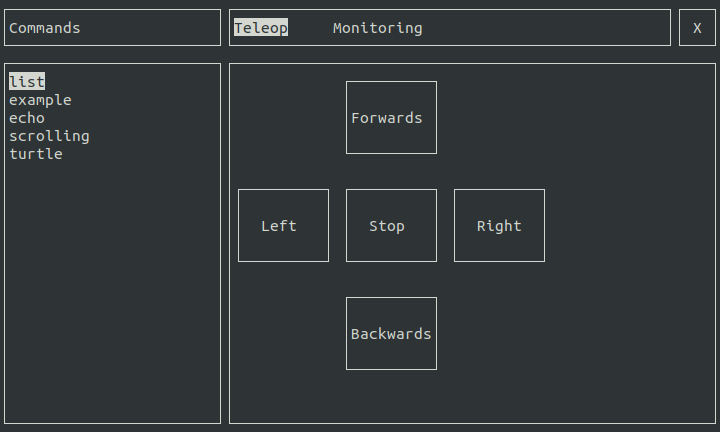
\includegraphics[scale=0.6]{Teleop}
  \caption{Screenshot of application showing the teleoperation interface}
  \label{fig:teleop}
\end{figure}

\newpage

The buttons themselves are sub-windows of the main output window. The reason for this is that it was easier to draw a box around them. Also, this makes it easier to determine if a mouse click was registered inside a button due to the {\fontfamily{pcr}\selectfont ncurses} function {\fontfamily{pcr}\selectfont wmouse}\_trafo. The function that defines the positions of each button is unfortunately long and overly complex. It also uses hard coded values for the button dimensions and the button labels. However, it effectively sizes the buttons appropriately and ensures that the label is kept in the middle of the button by forcing the vertical size to be an odd number.

In order to integrate the teleoperation tab into the tab bar, it was decided to keep it as the first index at all times. The menu printing function was modified to accept an extra vector of strings to prefix the start of the list. Additionally, it was hard coded that if the bar index was at 1, this indicated that teleoperation mode was active.

The user interface responds to teleoperation mode by displaying the teleoperation tab in the main window. Additionally, this allows the user to control the robot using the keyboard or on-screen buttons.

\subsection{Monitoring Tab}
\label{monitor_ui}

As explained in Section \ref{monitoring}, the monitoring tab was created as a static output displaying pre-defined sets of data. The UI comprises of two sections (Telemetry and Safety) containing lists of message data with preceding labels. As the interface is hard coded, the method of printing is not exactly elaborate, apart from the way that coloured boxes are displayed.

Colour-coded boxes are used for some items as opposed to raw data for a more visual representation of the robot status. This works by defining colour pairs for green, yellow and red, and assigning each to numbers. The number that is used is then based on the message value provided. As a precaution, any number outside of the expected range is treated as green by default. A box is then drawn by enabling the correct colour pair before printing two spaces which creates a square. A screenshot of the final version is shown below:

\begin{figure}[h!]
  \centering
  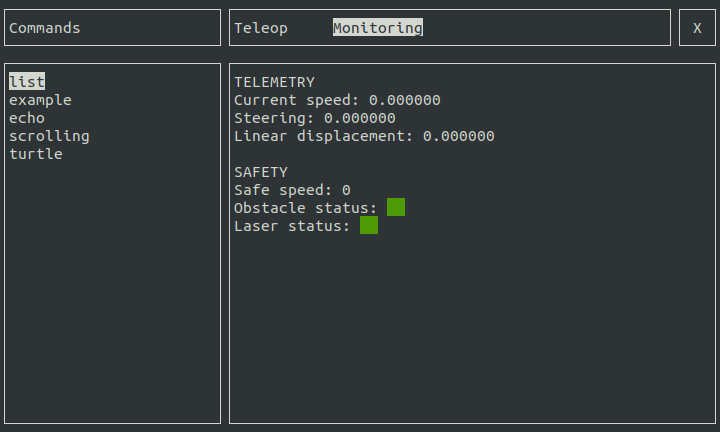
\includegraphics[scale=0.6]{Monitor}
  \caption{Screenshot of the monitoring interface}
  \label{fig:monitor}
\end{figure}

\section{Process Management}
\label{process_management}

\subsection{Starting Processes}
\label{starting_processes}

The application reads the {\fontfamily{pcr}\selectfont YAML} configuration file during its initialisation. Part of this file defines the commands to be made available in the menu and run within the program. The file is parsed using {\fontfamily{pcr}\selectfont yaml-cpp}\cite{yaml-cpp} and each process is constructed with the data extracted from there. The file was originally using a custom format until it was decided that this would be too complicated and unnecessary. Also {\fontfamily{pcr}\selectfont YAML} is used heavily in {\fontfamily{pcr}\selectfont ROS} so using it for this application seemed more suitable than alternatives for the sake of consistency. Additionally, {\fontfamily{pcr}\selectfont yaml-cpp} is the actual library used by {\fontfamily{pcr}\selectfont ROS} to interpret {\fontfamily{pcr}\selectfont YAML} files. This means that on some systems, there is no need to install it as a separate dependency (although this was not consistently true). It was also decided to separate the program executable option from the parameter option in the file. This makes parsing easier due to the increased ability to deal with commands that do not use parameters.

The location of the {\fontfamily{pcr}\selectfont YAML} file is initially presumed to be in the ".config" directory as this is standard for most Unix applications. However, if this is not present, the provided sample file is read as a temporary alternative.

In order to start a process, the strings in the {\fontfamily{pcr}\selectfont YAML} file need to be split in order to extract the executable name and the separate parameters to be passed to {\fontfamily{pcr}\selectfont execv}\cite{exec}. This was done using the {\fontfamily{pcr}\selectfont boost}\cite{boost} split algorithm, splitting by spaces or "/" characters where appropriate. This was planned to be done manually using {\fontfamily{pcr}\selectfont strtok}, however, due to complications, it was decided to make use of pre-made libraries. This made the relevant sections of code simpler and ultimately saved development time. There were also some initial problems regarding accepting zero or multiple parameters. However, these were alleviated by making use of both {\fontfamily{pcr}\selectfont yaml-cpp} and the {\fontfamily{pcr}\selectfont boost} split algorithm and is now functioning properly.

When the necessary process information has been extracted from the configuration file, the desired process is run when it is selected from the menu. This is done by forking the program and running the {\fontfamily{pcr}\selectfont execv} function. Specifically, the program uses {\fontfamily{pcr}\selectfont forkpty}\cite{forkpty} which forks as well as creates a new pseudo-terminal simultaneously. This streamlines the common practice of doing this manually with arguably verbose code. Before introducing pseudo-terminals as described in Section \ref{section:pty}, the regular {\fontfamily{pcr}\selectfont fork} function was used originally before the change in design decision.

\subsection{Emulating Teletype Interfaces}
\label{section:pty}

An unforeseen issue surfaced while testing the application using {\fontfamily{pcr}\selectfont ROS} commands such as {\fontfamily{pcr}\selectfont roscore} and {\fontfamily{pcr}\selectfont roslaunch}. This issue was primarily to do with how {\fontfamily{pcr}\selectfont ROS} utilities (as well as other programs) display and manipulate data in the terminal. In order to display text in colour without explicitly using ASCII escape codes, as well as accept standard input as raw input, these programs change the {\fontfamily{pcr}\selectfont termios} attributes of their respective terminal devices. If a program does this to suit its own needs, the parent application does not accept user input as the {\fontfamily{pcr}\selectfont ncurses} settings were being overridden by the children.

The solution to this problem was to essentially emulate a Teletype interface {\fontfamily{pcr}\selectfont (TTY)} using pseudo-terminals {\fontfamily{pcr}\selectfont (PTY's)}\cite{pty} for each child process so that they act as if they are running in a regular terminal environment. Additionally, it was necessary to disable standard input for each {\fontfamily{pcr}\selectfont PTY} so that the parent can take over. Much of the understanding and the actual code for this came from a project called {\fontfamily{pcr}\selectfont tty8}\cite{tty8}, an example of which can be found in Appendix \ref{appendix:c}.

The example shown illustrates how standard input as well as blocking were disabled as the process was being started. As well as this, during the creation of the {\fontfamily{pcr}\selectfont PTY}, the original signal mask was passed as a parameter in order to preserve the terminal attributes of the parent. This resulted in a positive outcome in which {\fontfamily{pcr}\selectfont ROS} processes were not interrupting the activity of the parent, allowing for effective multitasking and the ability to use the application as intended.

A subsequent benefit of this problem being solved was that the colour data that {\fontfamily{pcr}\selectfont ROS} outputs was being captured in its raw form where previously it was being omitted from the text. This creates the opportunity to parse and convert text into its intended colour in the main output screen using {\fontfamily{pcr}\selectfont ncurses} colour pairs during the printing stage. Unfortunately, due to time constraints this was not implemented and instead the codes are deleted using a regular expression. This makes use of the {\fontfamily{pcr}\selectfont regex}\cite{cpp-regex} standard library and does remove most of the undesired meta-data. There are some matches that are not consistent with other testing that was performed using a {\fontfamily{pcr}\selectfont regex} tester\cite{regex-tester} for unknown reasons. As a result there are some visible escape codes that are not too noticeable but are not removable for some unknown reason.

Another improvement that using pseudo-terminals made was the resolution of an issue identified during earlier development. The issue occurred when there were multiple tabs open and the user closes a tab that is to the left of any other tab. This resulted in the output of the tab that was to the right of the closed tab to stall indefinitely. The issue was non-existent after introducing pseudo-terminals even though the direct cause was never determined.

One problem with the way pseudo-terminals were being created was discovered later in development and was found to be the cause of major issues. Essentially, the original terminal settings that were passed to {\fontfamily{pcr}\selectfont forkpty} was being stored before the {\fontfamily{pcr}\selectfont ncurses} environment was initialised. This means that it was not using the terminal attributes set by {\fontfamily{pcr}\selectfont ncurses} but rather the settings used before initialisation. This, combined with not properly setting signal settings on the side of the parent, lead to undefined behaviour and complete crashing. This usually occurred when trying to use the mouse as described in Section \ref{sidebar_menu} and made any hope of using the mouse potentially dangerous. The issue was also leading to inconsistent output behaviour such as randomly making all output upper-case. The issue has since been properly resolved and the mouse input behaves as expected.

\subsection{Capturing Process Output}
\label{capturing_output}

An initial design decision was to use {\fontfamily{pcr}\selectfont popen}\cite{popen} in order to combine forking and running {\fontfamily{pcr}\selectfont exec} and {\fontfamily{pcr}\selectfont fdopen}\cite{fdopen} into one function. However, due to a misunderstanding as to how {\fontfamily{pcr}\selectfont popen} works, it was found to be unhelpful for certain features of the application. The reason for this is that {\fontfamily{pcr}\selectfont popen} does not return the process ID of the forked process which means that it is impossible to reliably kill it. The only way to use this would be to kill processes with {\fontfamily{pcr}\selectfont pkill}\cite{pkill} which kills all processes matching a regular expression which is not ideal. This meant that it was necessary to re-implement the functionality of {\fontfamily{pcr}\selectfont popen} in order to gain access to both the standard output and the {\fontfamily{pcr}\selectfont PID} of each process. This served to delay development as well as make the code more complicated than initially predicted. However, this re-implementation meant that solving a later issue \ref{section:pty} was easier due to more granular control over the functionality.

In order to display process output properly, it needs to be redirected, captured and stored appropriately. This was done using {\fontfamily{pcr}\selectfont fdopen} to create a file stream that captures the file descriptor of a pseudo-terminal. This is done for each respective process that is run. In order to get the data from the file stream, {\fontfamily{pcr}\selectfont fgets} was used as it terminates either at a newline character or after a specified amount of characters. This is helpful because if the size of the window is given to it, this results in line wrapping built in to the function. This is performed for every process in the tab bar iteratively. An example of line wrapping is shown in the screenshot below:

\begin{figure}[h!]
  \centering
  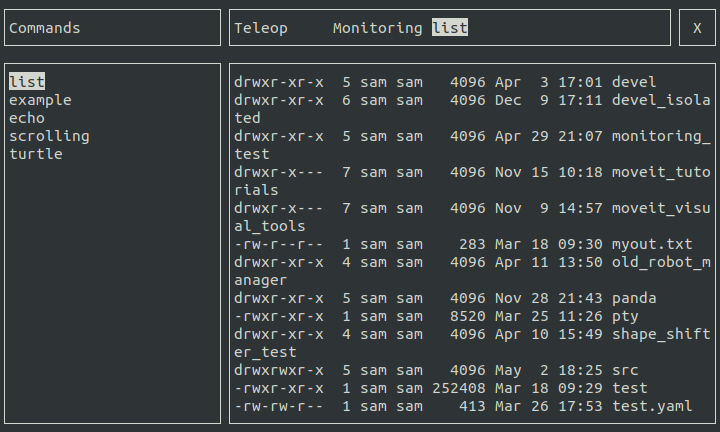
\includegraphics[scale=0.6]{TrueOutput}
  \caption{Screenshot of the {\fontfamily{pcr}\selectfont ls} program output being displayed and wrapped}
  \label{fig:output}
\end{figure}

Before the implementation of pseudo-terminals as described in Section \ref{section:pty}, the output redirection was being done with pipes and the {\fontfamily{pcr}\selectfont dup2} function. There were some initial issues with redirecting the file descriptors correctly as it is not well explained in the documentation. Also, before the discovery of the {\fontfamily{pcr}\selectfont fdopen} utility, there was an attempt to recreate {\fontfamily{pcr}\selectfont fgets} using the read function. This turned out to be a waste of time and was not successful regardless of the inclusion of {\fontfamily{pcr}\selectfont fdopen}.

\subsection{Killing Processes}
\label{killing}

An integral and simultaneously temperamental aspect of this project is to be able to kill processes easily. The way this was being done initially was to send a kill signal using {\fontfamily{pcr}\selectfont SIGINT} and then wait for the given process to terminate. The advantage of this is that the program can take note of the death of a process and prevent it from remaining in a zombie state. However, a particular problem with {\fontfamily{pcr}\selectfont ROS} applications is that they need to shut down safely and thus take a long time to terminate. The result of this is that the parent application that is waiting for them to terminate is completely frozen. However, since learning about options that can be passed to {\fontfamily{pcr}\selectfont waitpid}, a subroutine was added to keep track of terminated processes and subsequently wait for each of them and remove them once each process has fully terminated. This made killing {\fontfamily{pcr}\selectfont ROS} processes safer, more reliable and less likely to halt the parent application.

\section{Teleoperation}
\label{teleop}

This section describes the back-end implementation of the teleoperation feature. The general function of this is to construct and send geometry twist messages to a given {\fontfamily{pcr}\selectfont ROS} topic. The message that is sent will be adjusted based on user input, changing the linear velocity and the turning increment. Each button press will add an amount to the relevant velocities in question.

In order to ensure that the robot can be straightened, it was made so the turning value will degrade to zero over time. This allows the robot to continue to drive in a straight line if no alterations are made. This occurs iteratively after a given amount of time and subtracts a given amount from the velocity before sending a message. Without this delay, it was found that turning is impossible due to the main loop being too fast.

If the stop function is called, a linear and rotational velocity of 0 will be published ten times. This was a suggested amount given by the project supervisor based on the behaviour of the systems already in place. Sending multiple stop messages simply ensures that at least one will be received by the robot and is a point of precaution.

One issue discovered during hardware testing was that velocity messages were being sent out far too quickly, leading to lag and a large message queue. This was due to the fact that messages were being re-sent during each iteration of the main loop without any sort of delay. Messages have to be sent constantly during teleoperation in order to maintain control, however the lack of delay was causing problems for other applications. The solution to this was to add a timer to the refresh function that will tick over after a configured amount of seconds. The value of the amount of time to wait is defined in the configuration file which gives the user the ability to adjust it according to the needs of the hardware being used. Additionally, it was found that the queue for the {\fontfamily{pcr}\selectfont ROS} publisher was too large at 100 and should have been set to 10 to further limit the amount of messages that are sent at any one time.

An emergent behaviour of having two message sending timers is that, of course only one of them is going to be useful. That would be the time that is the smallest which does make the second timer redundant. That being said, the functionality of each is technically different given that one timer reduces rotational velocity as well as sends messages. So, depending on the system, it may be worth setting one higher than the other, meaning that the option is there if needed.

Much of the teleoperation behaviour is dependent on the configuration file as it defines the following attributes:

\begin{itemize}
  \item The amount of time to wait between sending regular messages
  \item The topic to publish to
  \item The magnitude of the rotational degradation
  \item The amount of time to wait between degrading the rotation
  \item The magnitude of the linear and rotational velocities to be added on for every button press
\end{itemize}

An example set of values can be viewed in the teleop section of the example configuration file in Appendix \ref{appendix:c}.

A feature that was also implemented was a teleoperation mode that would disable when not on the teleoperation tab of the interface. Disabling this mode means that no messages will be sent which allows other {\fontfamily{pcr}\selectfont ROS} processes to take control of the robot without interruption. There was an issue with this function where, while switching tabs will send a stop signal, the previous velocity before the switch was somehow being stored. This lead to the robot resuming movement when switching back to the teleoperation tab. This issue was solved by sending more stop signals and being more strict when entering and leaving teleoperation mode.

An unfortunate consequence of having one application that can control robots as well as manage processes is that it still has to be a {\fontfamily{pcr}\selectfont ROS} node. As such, it requires {\fontfamily{pcr}\selectfont roscore} to be running before it is started which is unfortunate as it means that the output of {\fontfamily{pcr}\selectfont roscore} cannot be monitored in a tab. This issue was discovered late in development and is unfortunately not fixable given the nature of {\fontfamily{pcr}\selectfont ROS}. A suggested solution was to use {\fontfamily{pcr}\selectfont roslaunch} to launch the application as it automatically runs {\fontfamily{pcr}\selectfont roscore}. Unfortunately, due to the way that {\fontfamily{pcr}\selectfont roslaunch} changes the terminal settings, the application simply froze and did not work at all.

\section{Monitoring}
\label{monitoring}

The monitoring interface was initially designed to be a variable number of tabs that could be configured extensively to display any {\fontfamily{pcr}\selectfont ROS} topic data. However, due to a combination of factors, the interface was implemented as a static layout that displays pre-defined message types. One reason for this was time constraints nearing the end of development as well as complications involving subscribing to generic message types. Syntactically, {\fontfamily{pcr}\selectfont ROS} has no way to do this in {\fontfamily{pcr}\selectfont C++} as the callback message parameter needs to have a declaration of its message type.

There was an attempt at using shapeshifters\cite{shapeshifter}, however, the dependencies for doing this were not functional. While accomplishing something similar to this is possible, it was decided to create a monitoring tab that was suitable enough for Idris. The topics to subscribe to are defined in the configuration file and messages are checked for iteratively in the main loop. The back end of this process not exactly complex, although there are some interesting front end concepts described in Section \ref{monitor_ui}.

\chapter{Testing}

%Detailed descriptions of every test case are definitely not what is required here. What is important is to show that you adopted a sensible strategy that was, in principle, capable of testing the system adequately even if you did not have the time to test the system fully.

%Provide information in the body of your report and the appendix to explain the testing that has been performed. How does this testing address the requirements and design for the project?

%How comprehensive is the testing within the constraints of the project?  Are you testing the normal working behaviour? Are you testing the exceptional behaviour, e.g. error conditions? Are you testing security issues if they are relevant for your project? 

%Have you tested your system on ``real users''? For example, if your system is supposed to solve a problem for a business, then it would be appropriate to present your approach to involve the users in the testing process and to record the results that you obtained. Depending on the level of detail, it is likely that you would put any detailed results in an appendix.

%Whilst testing with ``real users'' can be useful, don't see it as a way to shortcut detailed testing of your own. Think about issues discussed in the lectures about until testing, integration testing, etc. User testing without sensible testing of your own is not a useful activity.

%The following sections indicate some areas you might include. Other sections may be more appropriate to your project. 

\section{Overall Approach to Testing}

As an agile project, tests evolved alongside the codebase as new features were introduced. Testing was conducted manually after each project build utilising a sample configuration file as well as various example programs (see Appendix \ref{appendix:c}). As a minimalist program, it was appropriate to perform full build tests regularly in order to test each individual feature as it is being developed. Once a feature is finished, the overall functionality of the existing system is evaluated. This ensures that implementing a new feature did not compromise what has already been done.

Usually when a bigger part of the software was to be added, a separate program with the same functionality of the subsystem was constructed and later integrated if it performed as expected. This is useful when using new technologies or when a section of code needs to be isolated in order to be tested. Isolation was necessary due to the fact that in ncurses, it is not possible to view output printed to the console during runtime as a form of debugging. The alternative to isolating code segments would be to change the printing function which did not always work due to the encapsulated, object-oriented nature of the design. This would also involve changing significant parts of the code and thus is not ideal.

Tests that involved interacting with robots were performed using a simulation, specifically {\fontfamily{pcr}\selectfont turtlesim}\cite{turtlesim}. This simulation listens to and interprets the same messages as the robots used in department in a similar way. It also runs well which is ideal for testing scenarios involving opening and closing the simulation as well as viewing {\fontfamily{pcr}\selectfont ROS} output which proved to be challenging at first . However, when the project was mature in its development, tests were being performed on actual hardware.

%\section{Regular Testing}

\section{Hardware Testing}

Opportunities for testing on real hardware were unfortunately limited and reserved for the end of the project. Testing was carried out using Idris as the screen was already working for that robot. Idris also has plenty of safety features to avoid accidental collisions. Other safety considerations and measures that were taken can be seen in Section \ref{safety}. The overall goal of this testing was mainly preparation for the final demonstration and assurance that everything would work without trouble. The aspects of the system that were tested are described in the following sections.

\subsection{All dependencies Satisfied}

There are a number of dependencies that are required at compile time such as {\fontfamily{pcr}\selectfont yaml-cpp} and the {\fontfamily{pcr}\selectfont boost} libraries, among others. The only dependency not satisfied at the time of testing was {\fontfamily{pcr}\selectfont yaml-cpp} which was then subsequently installed on Idris.

\subsection{Successful Code Compilation}

There were no issues here aside from an error regarding the minimum version of CMake required. This was resolved by simply changing the requirements in the CMake configuration file.

\subsection{User Interface Displaying Properly}
\label{ui_display_prop}

In some terminal emulators, the user interface does not display as it should. This is potentially due to character encoding errors. Prior to testing on Idris itself, the application was tested in various terminal environments, the results of which are shown below:

%\begin{itemize}
  %\item {\fontfamily{pcr}\selectfont st}\cite{st} - PASSED
  %\item {\fontfamily{pcr}\selectfont xterm}\cite{xterm} - PASSED
  %\item {\fontfamily{pcr}\selectfont urxvt}\cite{urxvt} - PASSED
  %\item The {\fontfamily{pcr}\selectfont GNOME} Terminal - PASSED
  %\item {\fontfamily{pcr}\selectfont Konsole} (KDE Terminal)\cite{konsole} - FAILED
  %\item A plain {\fontfamily{pcr}\selectfont TTY} running on {\fontfamily{pcr}\selectfont Arch}, {\fontfamily{pcr}\selectfont Parabola} and {\fontfamily{pcr}\selectfont Ubuntu}  Linux - PASSED
  %\item {\fontfamily{pcr}\selectfont Tmux} running in a plain {\fontfamily{pcr}\selectfont Ubuntu} TTY - PASSED
%\end{itemize}

\begin{table}[h!]
  \centering
  \begin{tabular}{| m{15em} | c |}
  \hline
  Test Environment & Pass/Fail \\
  \hline
    {\fontfamily{pcr}\selectfont st}\cite{st} & Pass \\
  \hline
    {\fontfamily{pcr}\selectfont xterm}\cite{xterm} & Pass \\
  \hline
    {\fontfamily{pcr}\selectfont urxvt}\cite{urxvt} & Pass \\
  \hline
    The {\fontfamily{pcr}\selectfont GNOME} Terminal & Pass \\
  \hline
    {\fontfamily{pcr}\selectfont Konsole} (KDE Terminal)\cite{konsole} & Fail \\
  \hline
    Plain {\fontfamily{pcr}\selectfont TTY} running on {\fontfamily{pcr}\selectfont Arch}, {\fontfamily{pcr}\selectfont Parabola} and {\fontfamily{pcr}\selectfont Ubuntu} Linux & Pass \\
  \hline
    Tmux running in a plain {\fontfamily{pcr}\selectfont Ubuntu TTY} & Pass \\
  \hline
\end{tabular}
  \caption{Test results of running application in various terminal emulators}
\end{table}

Idris is running a plain {\fontfamily{pcr}\selectfont TTY} in {\fontfamily{pcr}\selectfont Gentoo} Linux which was able to display the application properly with no issues. There were also concerns regarding whether or not the sidebar would be too big as the width is hard coded and the mounted screens are reasonably small. However, the resolution of the screen was appropriately sized meaning that all output in each window looked sensible.

\subsection{Processes Terminating Correctly}

The particular processes used on Idris had not yet been tested (nor were they known exactly beforehand) and so it was important to test managing them. This provides a good example of a real life scenario. Due to one of the issues outlined in Section \ref{killing}, it was discovered through this testing that waiting for a process to close was causing problems. This lead to multiple processes having to be painstakingly killed manually from a separate computer.

\subsection{Appropriate Signals Sent from the Teleoperation Tab}

This test lead to the discovery of the issue detailed in Section \ref{teleop} regarding the teleoperation tab sending too many signals in rapid succession. The consequence of this was very noticeable latency when monitoring the velocity topic using {\fontfamily{pcr}\selectfont rostopic echo}.

\section{User Interface Testing}

The UI was tested using some example programs in Appendix \ref{appendix:c}, most notably the second example. This helped to test how the scroll bars were being drawn as well as scrolling in general by changing the amount of lines printed. Additionally, some third party programs were used such as the {\fontfamily{pcr}\selectfont GNU ls} command as well as {\fontfamily{pcr}\selectfont neofetch}\cite{neofetch}. The {\fontfamily{pcr}\selectfont ls} command was used as a simple test with a usually small output stream that was guaranteed to stop outputting new lines. {\fontfamily{pcr}\selectfont Neofetch} was used for similar reasons as well as having the ability to test how colour output is dealt with. 

{\fontfamily{pcr}\selectfont Neofetch} changes several attributes (such as coloured and bold text) for some lines, creating several instances of concatenated escape codes which is an unusual test case for omitting these codes generally. This served to test how robust the printing and output capturing systems were due to its complexity. These programs were included in the configuration file and were run as part of regular testing for new features.

\section{Stress Testing}

The application is deliberately very minimal in order to deal with multiple process output streams without impacting performance. However, processing this output is done in real time in one loop so stress testing the refresh rate of the program is important. The main form of stress testing employed was an example program in Appendix \ref{appendix:c} which prints numbers incrementing from 0 to any arbitrary amount infinitely. Several instances of this program were run at one time within the application. This allowed for testing the refresh rate of the printing function as well as how the program dealt with updating several tabs at a high refresh rate. 

There used to be no delay used in this program so the update rate was as fast as the hardware allowed it. However, this lead to 100\% of the CPU thread being used during testing and was dealt with using a five millisecond delay. A higher delay makes the interface feel sluggish and any smaller delay greatly increases the load on the CPU. The current load sits at approximately 20\% on an {\fontfamily{pcr}\selectfont Intel i7 4790K} at {\fontfamily{pcr}\selectfont 4.4GHz} running {\fontfamily{pcr}\selectfont Ubuntu}.

\section{User Testing}

Each sprint focused on delivering demonstrable features that have an observable impact on the application from the perspective of the user. At the end of a sprint, during the weekly meeting with the project supervisor (who is also the client), there was an opportunity for them to try newly developed features on a laptop. Although, later in the project, this became impossible as the application required {\fontfamily{pcr}\selectfont ROS} in order to run which was not installed on said laptop. This was mainly due to the difficulty of installing {\fontfamily{pcr}\selectfont ROS} on Linux distributions not based on {\fontfamily{pcr}\selectfont Ubuntu} such as {\fontfamily{pcr}\selectfont Arch}.

The replacement for this was to show screen casts of the new features alongside commentary and further discussion. These screen casts included a log of every keystroke using {\fontfamily{pcr}\selectfont screenkey}\cite{screenkey} in order to make it clear what is happening in the video. These demonstrations usually lead to new features/requirements being added due to a better understanding of how the software was developing from a usability perspective. User tests were deliberately frequent and varied in order to respond to change more effectively and to test the latest and more appropriate aspects of the system.

\chapter{Evaluation}

%Examiners expect to find a section addressing questions such as:

%\begin{itemize}
   %\item Were the requirements correctly identified? 
   %\item Were the design decisions correct?
   %\item Could a more suitable set of tools have been chosen?
   %\item How well did the software meet the needs of those who were expecting to use it?
   %\item How well were any other project aims achieved?
   %\item If you were starting again, what would you do differently?
%\end{itemize}

%Other questions can be addressed as appropriate for a project. 

%The questions are an indication of issues you should consider. They are not intended as a specification of a list of sections.

%The evaluation is regarded as an important part of the project report; it should demonstrate that you are capable not only of carrying out a piece of work but also of thinking critically about how you did it and how you might have done it better. This is seen as an important part of an honours degree. 

%There will be good things in the work and aspects of the work that could be improved. As you write this section, identify and discuss the parts of the work that went well and also consider ways in which the work could be improved. 

%In the latter stages of the module, we will discuss the evaluation. That will probably be around week 9, although that differs each year. 

\section{Evaluation of Agile Approach}

Due to the uncertainty of how the requirements would manifest as well as the knowledge that plans would inevitably change, an agile approach seemed most appropriate. This initial decision proved to be most effective as it allowed for rapid prototyping and proving concepts before moving forward with potentially uninformed rigorous design. This was also closely aligned with the fact that meetings with the project supervisor occurred regularly and frequently. Given that the supervisor was also the client/user of the application, it was suitable to show regular prototypes as a form of user testing. The ability to respond to change combined with the technical experience of the project supervisor meant that the correct decisions were taken even without a formal design.

\section{Identifying the Requirements}

The requirements in Section \ref{user_stories} were identified at the start of the project and remained consistent throughout the project. However, these requirements do not describe the entire system in detail as they are specifically user-oriented stories. The advantage of this is a greater focus upon implementation time, however, the downside is the lack of direction from the offset. This could have been improved and may have helped to mitigate issues faced during development. However, the approach was (and is) viewed as more appropriate for the individual project undertaken.

\section{Design Decisions}

As an agile projects, it was expected that some design decisions would have to be remedied later on in the project. This is due to change in requirements from the client, dealing with integration issues or responding to a change in understanding of the technologies used. Such examples have been documented in earlier sections, namely \ref{implementation_tools}, \ref{ui_design}, \ref{section:pty} and \ref{capturing_output}. However, these issues were appropriately dealt with and are only a subset of design decisions that were made. Other various decisions outlined in previous sections such as \ref{other_decisions} required no changes and the substance of what was produced suffered no ill effects due to design.

\section{Appropriateness of Tools Used}

The C++ language was the most appropriate tool due to the reasons outlined in Section \ref{implementation_tools}. The decision to use ncurses was also appropriate over the other alternative tools noted in Section \ref{reading_and_prep}. It is certainly more appropriate than any graphical library for the purposes of the project, despite its low-level and verbose nature.

In terms of editing tools, the choice to use neovim over a more fully featured IDE arguably had some impact on development time. However, the only tangible benefit gained from using an IDE for this project is automatic code completion and refactoring. Using any integrated console is unsuitable as it would make it harder to view the application running. This means that many of the features of an IDE would be unavailable without spending time trying to make it work. Neovim and other similar editors are also much faster regardless of hardware specifications in many cases. Therefore, the appropriateness of this tool is not entirely non-existent.

The appropriateness of using YAML as well as the yaml-cpp library is noted in Section \ref{starting_processes}. Using other formats or creating a custom parser would have been less suitable and more time consuming.

\section{Relevance to Degree Scheme}

The relevance of this project to my degree scheme (Artificial Intelligence and Robotics) was questioned before the start of the semester. This was primarily due to the lack of robotics involved in the initial specifications of the project. The argument was made that it was more associated with either a software engineering or system management project. Even if the application will be running on robots, the substance of the task did not involve interacting with them them. Due to this decision, it was decided to include additional requirements. These were to create a way to operate the robot from the application as well as display ROS topic information.

\section{Application and Impact}
\label{application}

As evidenced by the relatively successful hardware testing as well as feedback from the project supervisor/client, the usefulness of the developed software is certainly apparent. The fundamental requirements were satisfied and function correctly and the application itself is easy to use and runs effectively. There were other discussions during meetings regarding optional features that would make the system more like a pseudo desktop environment. Features such as colour-coded tabs and tabs being opened using specified shortcut keys would definitely add to the overall usability of the application. However, these features were strictly classified as optional and were reserved for the end of the project if there was any spare time remaining.

The impact of the completion of this project has the potential to be very beneficial for day-to-day research, providing more flexibility and redundancy for controlling the rovers. There is also the possibility of this software being used for other non-robotics systems if the ROS features were removed and the terminal emulation was more robust. It can be used for demonstrations or possibly a normal terminal multiplexer with built-in executable shortcuts.

\section{Time Management}

At the beginning of a sprint, tasks were chosen in accordance with the assessment of velocity. As a result, it was foreseen how much should be completed within the sprint which provided a measure of how well time was being managed. On a day-to-day basis, due to the ability to carry out work at any location (ie. from home) for most of the project, it was possible to start working first thing in the morning. This provided motivation to complete more work as the day progressed and resulted in more intense focus on the allotted tasks at hand. There were unfortunately long periods where little to work was completed due to illness. However, on days where the usual methods of working were not sufficient, techniques such as the pomodoro technique\cite{pomodoro} were employed to help manage time.

There was no use of a schedule which has advantages and disadvantages. The obvious disadvantage is the inherent disorganisation that comes with a lack of a formal schedule. However, an advantage of this is the ability to have more intense focus on the project as a whole instead of constantly switching between tasks. Also, this approach provides plenty of opportunity to prioritise and re-organise work if this is indeed necessary. These reasons create a time management methodology that maintains focus and ultimately fits into the agile nature of the project.

Due to these methods, time management was adequate enough to finish the main project. However, some steps could have been taken to manage time more effectively with more order and organisation to the day. That being said, what was employed was suitable and necessary for me as an individual as opposed to alternative approaches that may not have provided any benefit to me.

%\section{What Could Have Been Done Differently}

%\begin{itemize}
%  \item More plan driven
%  \item Better time management
%  \item More formal testing procedures
%  \item More in-depth background reading
%\end{itemize}

\section{Future Work}

As noted in Section \ref{application}, there is the potential for this system to be a fully complete terminal emulator with its own truly unique features. The elements to be addressed in order to achieve this are noted below:

\subsection{Extra Usability Features}

Section \ref{application} describes optional features that were suggested such as shortcut keys. Providing other way to interact with the application can make it more usable as a replacement for a graphical desktop environment. This is important for both other use cases as well as the intended use on robots if it is used for long periods of time.

\subsection{Signal Handling}

The application currently only displays standard output and standard error. There is no way to accept standard input from a child process as this was not necessary for the original intended purpose. This is the main reason why it is ineffective as a terminal emulator and would take high priority on the list of additions. There are also many other signals to emulate which would have been impossible to implement within the scope of the project.

\subsection{More Customisability}

The key-bindings are currently hard coded and are not configurable. This would be a valuable feature to add in order to accommodate for different user preferences. Also, there should be multiple keys mapped to the same function so that people collaborating can use their own layouts simultaneously without confusion.

Also, due to time constraints, the monitoring tab is hard coded which means that it is potentially useless on other machines without the same messages. An ideal system would allow easy customisation using any potential message type with any number of menu items.

\subsection{Help Menu}

Something that was brought up during testing was the addition of a help menu for new users. This is somewhat related to the lack of key customisation as different users will expect different default settings based on their own experience.

% add any additional chapters here

%TC:ignore
\setemptyheader

\nocite{*} % include everything from the bibliography, irrespective of whether it has been referenced.

% the following line is included so that the bibliography is also shown in the table of contents. There is the possibility that this is added to the previous page for the bibliography. To address this, a newline is added so that it appears on the first page for the bibliography. 
\addcontentsline{toc}{chapter}{Annotated Bibliography} % Adds References to contents page

%
% example of including an annotated bibliography. The current style is an author date one. If you want to change, comment out the line and uncomment the subsequent line. You should also modify the packages included at the top (see the notes earlier in the file) and then trash your aux files and re-run. 
%\bibliographystyle{StylesAndReferences/authordate2annot}
\bibliographystyle{StylesAndReferences/IEEEannotU}
\renewcommand{\bibname}{Annotated Bibliography} 

%\bibliography{StylesAndReferences/references} % References file
%\bibliography{~/Documents/bibliography} % References file
\bibliography{StylesAndReferences/bibliography} % References file


\setemptyheader

\addcontentsline{toc}{chapter}{Appendices}
\chapter*{Appendices}
%The appendices are for additional content that is useful to support the discussion in the report. It is material that is not necessarily needed in the body of the report, but its inclusion in the appendices makes it easy to access. 

%For example, if you have developed a Design Specification document as part of a plan-driven approach for the project, then it would be appropriate to include that document as an appendix. In the body of your report you would highlight the most interesting aspects of the design, referring your reader to the full specification for further detail.

%If you have taken an agile approach to developing the project, then you may be less likely to have developed a full requirements specification. Perhaps you use stories to keep track of the functionality and the 'future conversations'. It might not be relevant to include all of those in the body of your report. Instead, you might include those in an appendix. 

%There is a balance to be struck between what is relevant to include in the body of your report and whether additional supporting evidence is appropriate in the appendices. Speak to your supervisor or the module coordinator if you have questions about this.

\pagebreak

% start the appendix - sets up different numbering
\fancypagestyle{plain}{%
%\fancyhf{} % clear all header and footer fields
\fancyhead[L]{Appendix\ \thechapter}
\fancyhead[R]{\leftmark}}

\appendix
\fancyhead[L]{Appendix\ \thechapter}
\fancyhead[R]{\leftmark}
\fancyhead[C]{}
\fancyfoot[C]{\thepage}
\renewcommand{\headrulewidth}{0.4pt}
\renewcommand{\chaptermark}[1]{\markboth{#1}{}}

\fancyhead[L]{Appendix\ \thechapter}
\fancyhead[R]{\leftmark}
\fancyfoot[C]{{\thepage} of \pageref{LastPage}}

% include any appendices here
\chapter{Third-Party Code and Libraries}

%If you have made use of any third party code or software libraries, i.e. any code that you have not designed and written yourself, then you must include this appendix. 

%As has been said in lectures, it is acceptable and likely that you will make use of third-party code and software libraries. If third party code or libraries are used, your work will build on that to produce notable new work. The key requirement is that we understand what your original work is and what work is based on that of other people. 

%Therefore, you need to clearly state what you have used and where the original material can be found. Also, if you have made any changes to the original versions, you must explain what you have changed. 

%The following is an example of what you might say. 

%Apache POI library - The project has been used to read and write Microsoft Excel files (XLS) as part of the interaction with the client's existing system for processing data. Version 3.10-FINAL was used. The library is open source and it is available from the Apache Software Foundation 
%\cite{apache_poi}. The library is released using the Apache License 
%\cite{apache_license}. This library was used without modification. 

%Include as many declarations as appropriate for your work. The specific wording is less important than the fact that you are declaring the relevant work.

Boost C++ Libraries - This was used to parse and split string data from a YAML file. Version 1.69.0 was used. The library is open source and is available from the Boost Organisation.
\cite{boost}. The library is released under the Boost license
\cite{boost-license}. This library was used without modification.

yaml-cpp library - This was used to parse a configuration file using the YAML syntax. Version 0.6.2 was used. The library is open source and is available from the yaml-cpp Github Page.
\cite{yaml-cpp}. The library is released under the MIT license
\cite{yaml-cpp-license}. This library was used without modification.

ROS - This was used to interact with robotic systems also running ROS. The library is open source and is available from the ROS Website.
\cite{ros}. The library is released under the 3-Clause BSD License
\cite{bsd-license-3}. This library was used without modification.

ncurses - This was used to develop a text-based user interface. The library is open source and is available from the ncurses homepage.
\cite{ncurses}. The library is released under a permissive MIT-style license
\cite{ncurses-license}. This library was used without modification.

\chapter{Ethics Submission}

%This appendix includes a copy of the ethics submission for the project. After you have completed your Ethics submission, you will receive a PDF with a summary of the comments. That document should be embedded in this report, either as images, an embedded PDF or as copied text. The content should also include the Ethics Application Number that you receive. 

\begin{figure}[!ht]
  
\includegraphics[scale=0.75]{EthicsSubmission01}
\end{figure}
\begin{figure}[!ht]
  
\includegraphics[scale=0.75]{EthicsSubmission02}
\end{figure}
\begin{figure}[!ht]
  
\includegraphics[scale=0.75]{EthicsSubmission03}
\end{figure}

\chapter{Code Examples}
\label{appendix:c}

%For some projects, it might be relevant to include some code extracts in an appendix. You are not expected to put all of your code here - the correct place for all of your code is in the technical submission that is made in addition to the Project Report. However, if there are some notable aspects of the code that you discuss, including that in an appendix might be useful to make it easier for your readers to access. 

%As a general guide, if you are discussing short extracts of code then you are advised to include such code in the body of the report. If there is a longer extract that is relevant, then you might include it as shown in the following section. 

%Only include code in the appendix if that code is discussed and referred to in the body of the report. 

\section{Altering Child IO Signals}

\begin{verbatim}

/*These are a modified versioa of functions taken from the tty8 project
Copyright (c) 2015 Dima Krasner*/

/*Found in the Process class*/
int flags = fcntl(pty,F_GETFL);
fcntl(pty, F_SETSIG, SIGRTMIN + 1);
fcntl(pty, F_SETFL, O_ASYNC | O_NONBLOCK | flags);     
fcntl(pty, F_SETOWN, pid);

/*Found in main*/
void setMask(sigset_t * m, sigset_t * o) {
  sigemptyset(m);
  sigaddset(m, SIGCHLD);
  sigaddset(m, SIGINT);
  sigaddset(m, SIGTERM);
  sigaddset(m, SIGWINCH);
  sigaddset(m, SIGRTMIN);
  sigaddset(m, SIGRTMIN + 1);
}
\end{verbatim}

\section{Example Configuration File}

This YAML file was used as testing data throughout the project.

\begin{verbatim}
command:
  - name: "list"
    exec: "/bin/ls"
    param: "-l"
  - name: "example"
    exec: "example"
  - name: "echo"
    exec: "/bin/echo"
    param: "Hello World"
  - name: "scrolling"
    exec: "scrolltest"
    param: "50"
  - name: "turtle"
    exec: "/opt/ros/melodic/bin/rosrun"
    param: "turtlesim turtlesim_node"

teleop:
  topic: "turtle1/cmd_vel"
  degradation: 0.01
  turning_increment: 0.5
  linear_increment: 2
  refresh_timeout: 0.5
  degradation_timeout: 0.05

monitoring:
  telemetry_topic: "/idris/telemetry"
  safety_topic: "/idris/safety_status"
\end{verbatim}

\section{Test Programs}

The following are example programs used for testing the main application and were written separately from it.

\subsection{Example Program 01}

\begin{verbatim}
/*An example program used for stress testing the application*/

#include <stdio.h>
#include <unistd.h>

int main() {
  int i = 0;
  while(1) {
    printf("%d\n",i);
    i++;
  }
}
\end{verbatim}

\subsection{Example Program 02}

\begin{verbatim}
/*An example Program used to test scrolling functionality*/

#include <stdio.h>
#include <stdlib.h>

int main(int argc, char * argv[]) {
  if (argc < 2)
    printf("No args\n");
  else {
    for(int i = 0; i < atoi(argv[1]); i++)
      printf("%d\n",i);
  }
  return 0;
}
\end{verbatim}

\subsection{Example Program 03}

\begin{verbatim}
/*An example program used for testing file reading and YAML parsing*/

#include <yaml-cpp/yaml.h>
#include <iostream>
#include <string>
#include <vector>
#include "Process.h"
#include "FileReader.h"

main() {
  FileReader reader("test.yaml");
  std::vector<Process> processes = reader.getProcesses();
  processes[0].start();
  while(1) {
    processes[0].refreshBuffer(100);
    for (auto it : processes[0].getBuffer()) {
      std::cout << it;
    }
  }
}
\end{verbatim}

\chapter{Diagrams}
\label{appendix:d}

  \begin{figure}[h!]
    \centering
    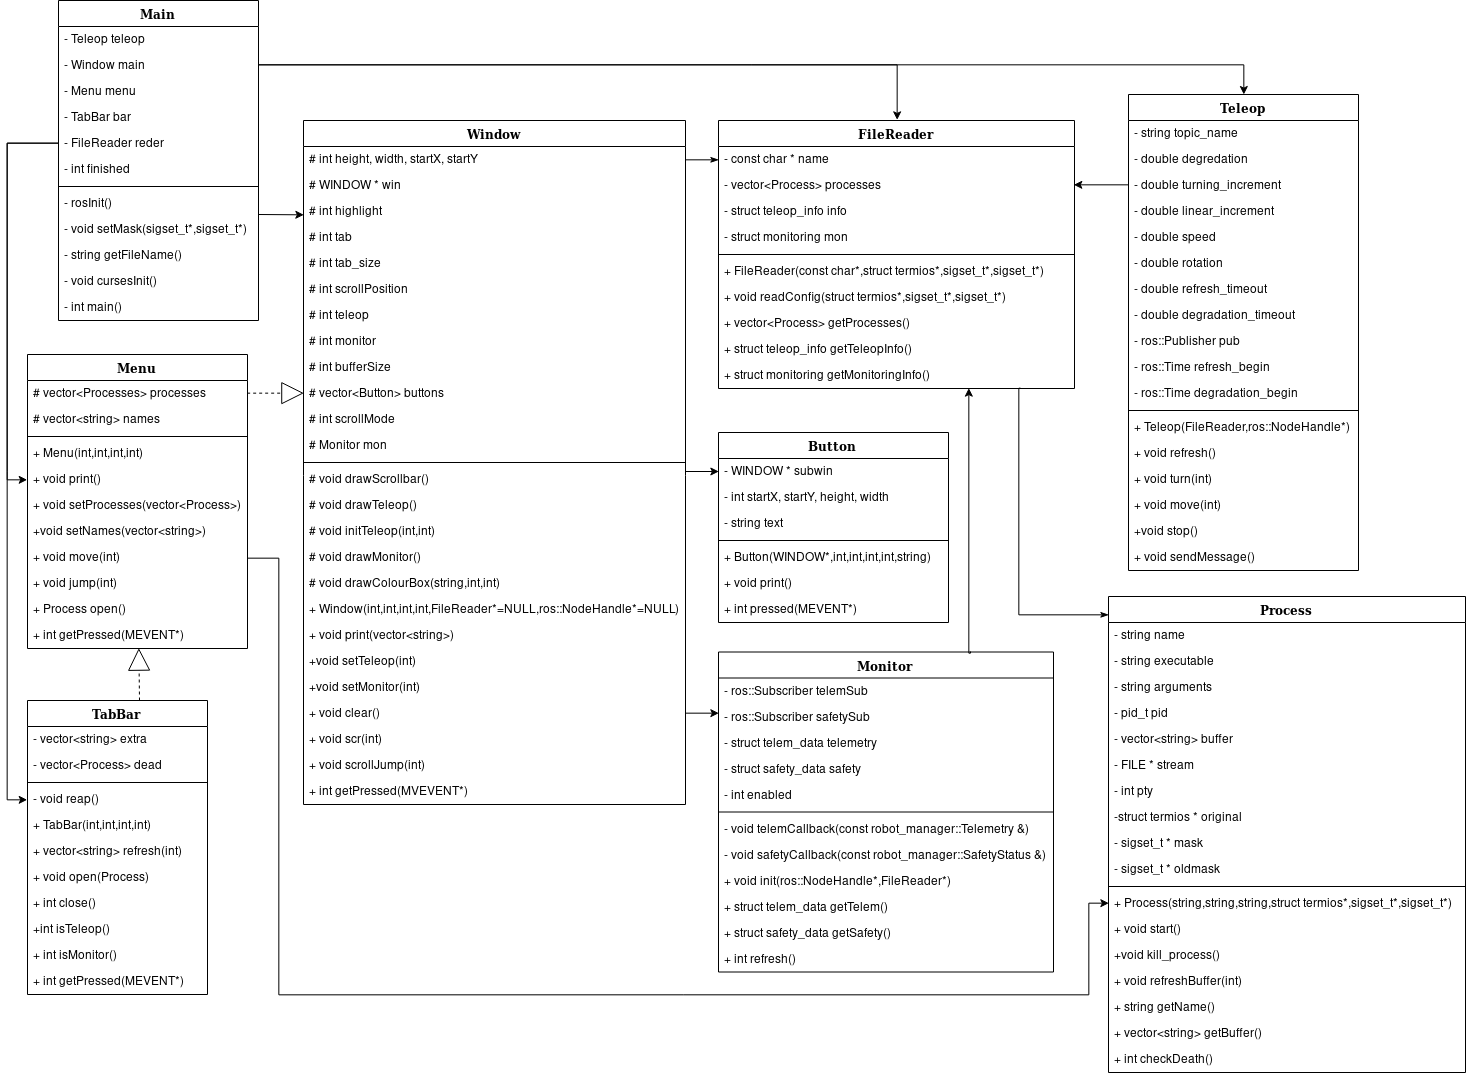
\includegraphics[scale=0.43,angle=-90]{ClassDiagramNew}
    \caption{UML class diagram of the final system}
    \label{fig:class-diagram}
  \end{figure}

  \begin{figure}[h!]
    \centering
    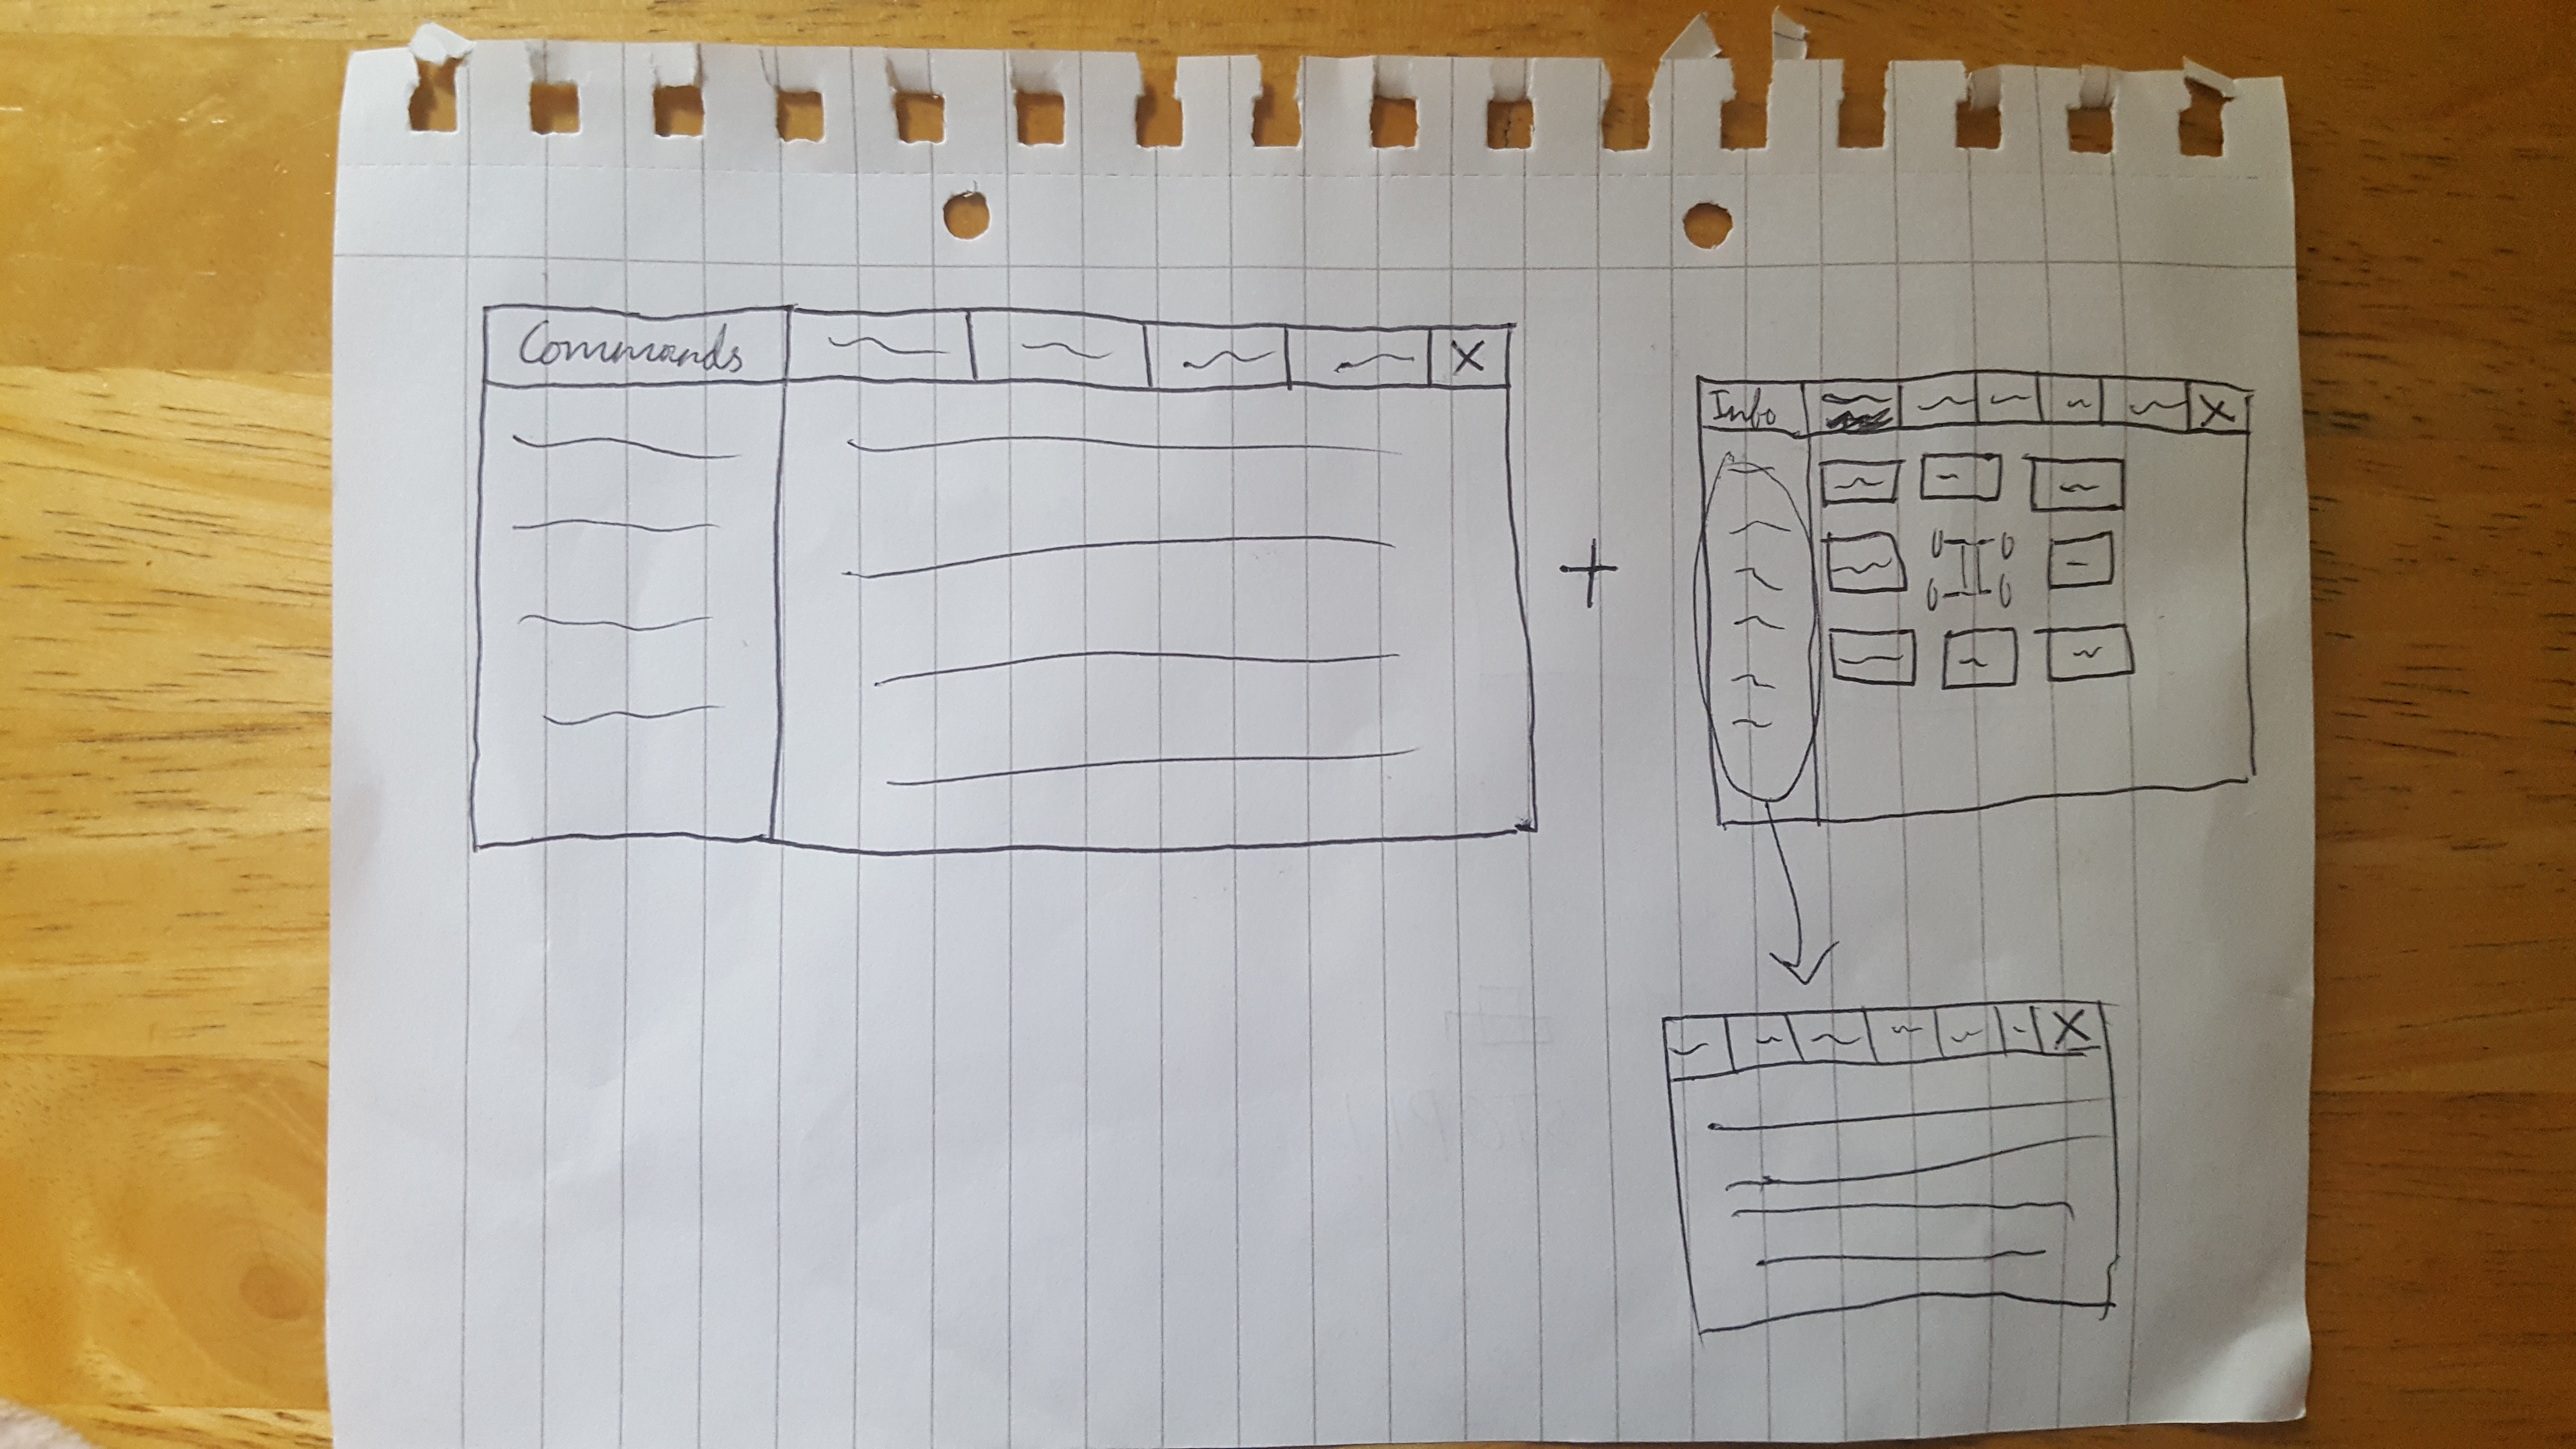
\includegraphics[scale=0.08]{UISketch01}
    \caption{Initial drawing of what the user interface was planned to look like}
    \label{fig:sketch01}
  \end{figure}

  \begin{figure}[h!]
    \centering
    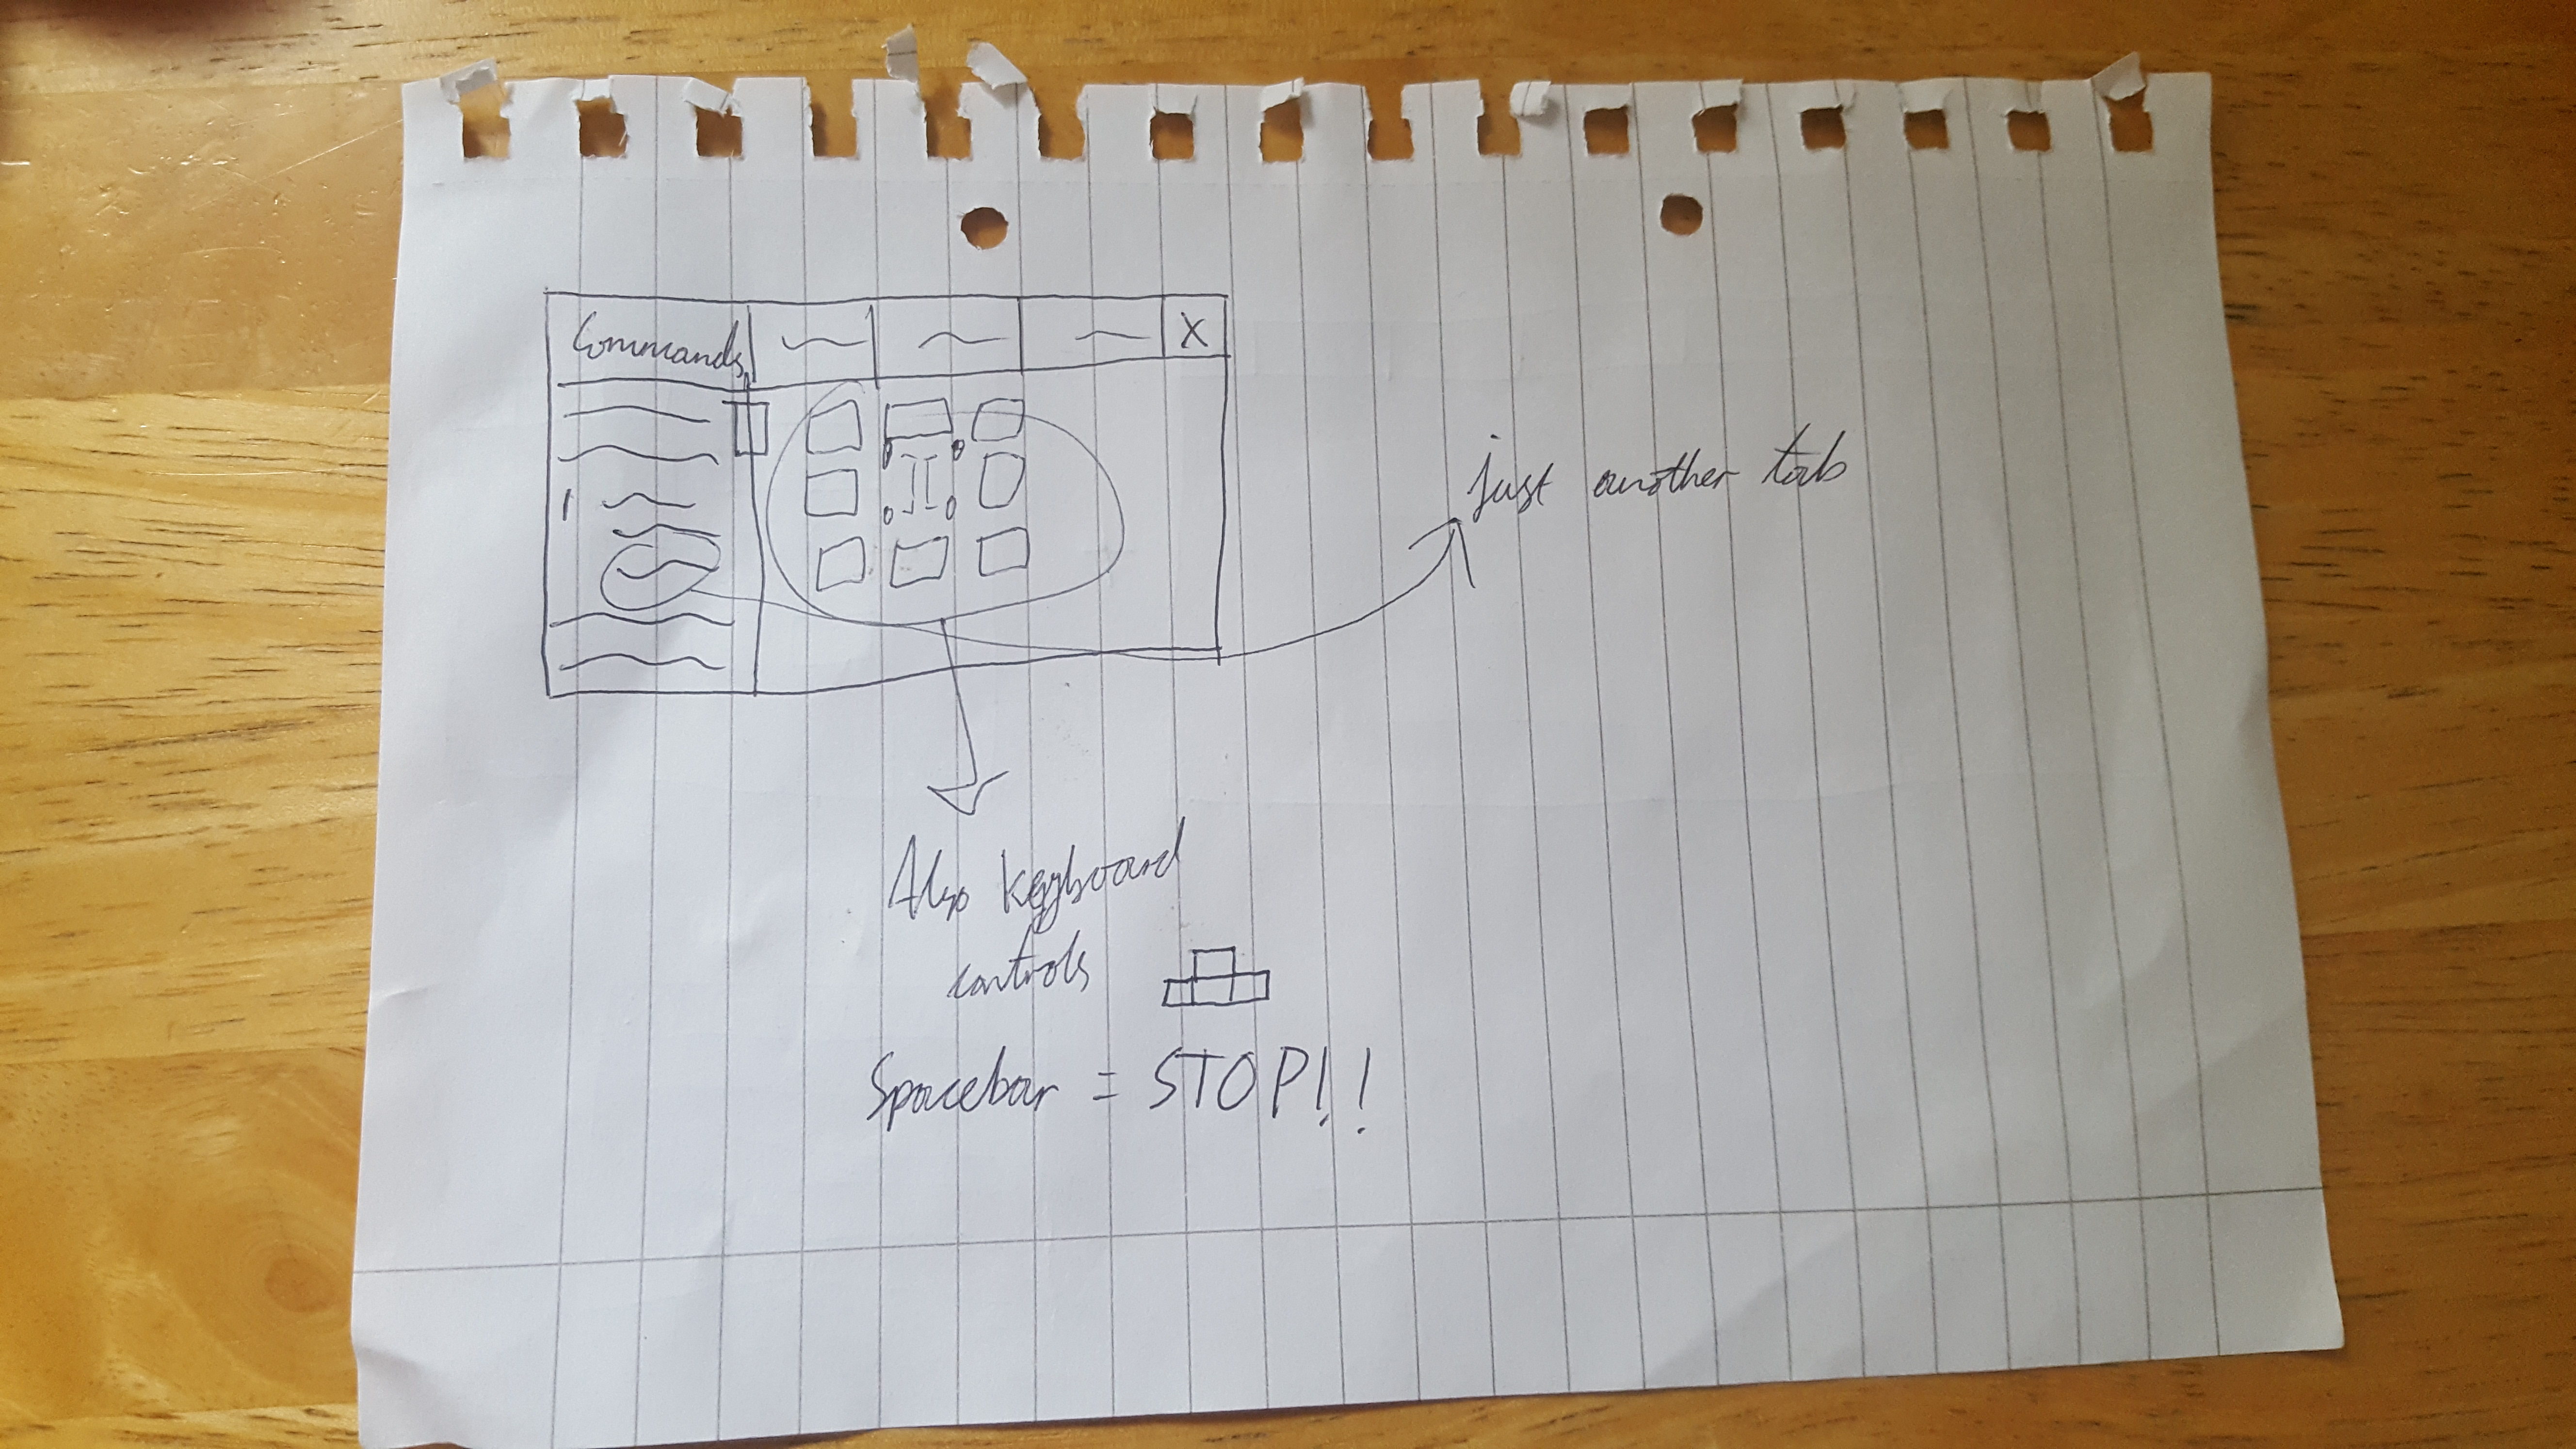
\includegraphics[scale=0.08]{UISketch02}
    \caption{Altered design to account for changes in client requirements and to have as much as possible on one screen}
    \label{fig:sketch02}
  \end{figure}


\fancypagestyle{plain}{%
   \fancyhead{} %[C]{Annotated Bibliography}
   \fancyfoot[C]{{\thepage} of \pageref{LastPage}} % except the center
   \renewcommand{\headrulewidth}{0pt}
   \renewcommand{\footrulewidth}{0pt}
}

%TC:endignore

\end{document}
